\documentclass[paper=a4, fontsize=11pt,x11names]{report}
\usepackage[T1]{fontenc}
\usepackage{fourier}

%margine a mano
\usepackage[margin=1.1in]{geometry}

\usepackage[utf8]{inputenc}
\usepackage[italian]{babel}
\usepackage[protrusion=true,expansion=true]{microtype}	
%\usepackage{amsmath,amsfonts,amsthm} % Math packages
\usepackage[pdftex]{graphicx}	
\usepackage{url}
\usepackage{graphicx}


%per il grafico
\usepackage{tikz}
\usepackage{tikz-er2}
\usetikzlibrary{positioning}
\usetikzlibrary{shadows}

\usetikzlibrary{mindmap,trees}
\usepackage{pgfplots} %per istorgrammi

\usepackage{float}

\usepackage{pdflscape}

%%% Custom sectioning
\usepackage{sectsty}
\allsectionsfont{\centering \normalfont\scshape}

%%% Custom headers/footers (fancyhdr package)
\usepackage{fancyhdr}
\pagestyle{fancyplain}
\fancyhead{}											% No page header
\fancyfoot[L]{}											% Empty 
\fancyfoot[C]{}											% Empty
\fancyfoot[R]{\thepage}									% Pagenumbering
\renewcommand{\headrulewidth}{0pt}			% Remove header underlines
\renewcommand{\footrulewidth}{0pt}				% Remove footer underlines
\setlength{\headheight}{13.6pt}

%\setlength{\textwidth}{6.5in}

%%% Equation and float numbering
%\numberwithin{equation}{section}		% Equationnumbering: section.eq#
%\numberwithin{figure}{section}			% Figurenumbering: section.fig#
%\numberwithin{table}{section}				% Tablenumbering: section.tab#




%%%%%%%%%%%%% per ER

\usepackage{tikz} 
\usetikzlibrary{er} 
\usetikzlibrary{arrows,automata}
\usetikzlibrary{positioning}
\tikzstyle{every entity} = [top color=white, bottom color=orange!20, 
                            draw=orange]
\tikzstyle{every weak entity} = [drop shadow={shadow xshift=.7ex, 
                                 shadow yshift=-.7ex}]
\tikzstyle{every attribute} = [top color=white, bottom color=MediumPurple1!20, 
                               draw=MediumPurple1]
\tikzstyle{every relationship} = [top color=white, bottom color=Chartreuse2!20, 
                                  draw=Chartreuse2]
\tikzstyle{every isa} = [top color=white, bottom color=yellow!20, 
                         draw=yellow]

%%%%%%%%%%%%%%%%%


%%% Maketitle metadata
\newcommand{\horrule}[1]{\rule{\linewidth}{#1}} 	% Horizontal rule


\title{
		%\vspace{-1in} 	
		\usefont{OT1}{bch}{b}{n}
		\normalfont \normalsize \textsc{Universit\`a degli Studi di Ferrara \\ Ingegneria Informatica e dell'Automazione
			\\ Basi di Dati} \\ [25pt]
		\horrule{0.5pt} \\[0.4cm]
		\Huge Realizzazione Database per Ospedale \date{}\\%[0.2cm]
		\horrule{0.5pt} \\[0.4cm]
		\LARGE Azzolini Damiano - Bertagnon Alessandro \\ [0.4cm]
		%\normalfont \normalsize Azzolini Damiano, Bertasi Francesco, Decarlo Dario, \\
		%\normalfont \normalsize Fazzi Mattia, Fiorini Giovanni, Fontana Niccol\`o, Rambaldi Marco\\[0.4cm]
		\horrule{2pt} \\[0.8cm]
		
\includegraphics{logoUnife}
		%\horrule{2pt} \\[0.5cm]
		%%%%%%%%%%%%%%%%%%%%%%%%%%%%%%% MANCA DATA %%%%%%%%%%%%%%%
}


%%% Begin document
\begin{document}
\maketitle

\newpage

\tableofcontents
\thispagestyle{empty}

%\listoffigures
%\thispagestyle{empty}


\newpage

\pagenumbering{arabic}
%\begin{abstract}
%Your abstract goes here...
%\end{abstract}

%\chapter{Introduction} %solo per report
%This chapter's content...


%%%%%%%%%%%%%%%%%%%%%%%%%%%%%%%%
%%%%%%%%%%%%%%%           \`u

%%%%%%%%%%%%%%%%%%%%%%%%%%% DESCRIZIONE MINIMONDO
\chapter{Minimondo}
\section{Descrizione}
Il progetto si basa sulla realizzazione di una applicazione web per la gestione di una clinica privata. Alla piattaforma possono accedere 5 tipi di utente:
\begin{itemize}
\item paziente
\item medico
\item infermiere
\item impiegato
\item amministratore
\end{itemize}  

La clinica in questione eroga diverse \textbf{prestazioni} ai suoi utenti, ad esempio: visite specialistiche, esami diagnostici, day surgery e terapie. Ogni prestazione può essere effettuata da uno o più membri dello \textbf{staff} (a seconda della complessità della prestazione stessa) in una delle \textbf{sale} della clinica. Al termine di ogni prestazione, il medico compila un \textbf{referto} corrispondente alla prestazione appena effettuata. Il sistema deve anche gestire i \textbf{farmaci} assunti dagli utenti e/o eventualmente utilizzati durante le prestazioni. Per motivi di organizzazione interna ogni membro del personale e ogni sala afferisce a uno specifico \textbf{reparto} della clinica. Ad ogni utente è associato un \textbf{Ruolo}, ovvero un insieme di azioni che esso può svolgere sulla piattaforma. I ruoli di base assegnati a ciascun utente dipendono dalla tipologia dello stesso e sono:\\

L'utente \textbf{PAZIENTE} potrà:
\begin{itemize}
\item Fare il login sulla piattaforma e modificare il proprio profilo.
\item Aggiungere/Rimuovere i farmaci che assume regolarmente.
\item Visionare le prestazioni effettuate con i referti corrispondenti.
\end{itemize}

L'utente \textbf{MEDICO} potrà:
\begin{itemize}
\item Fare il login sulla piattaforma e visionare il proprio profilo.
\item Registrare nuovi pazienti sulla piattaforma.
\item Visionare le schede personali dei pazienti (compresi i farmaci assunti).
\item Visionare le prestazioni assegnategli e i relativi referti.
\item Aggiungere il referto ad una prestazione a cui ha preso parte.
\item Aggiungere/Rimuovere i farmaci utilizzati nelle prestazioni a cui ha preso parte.
\item Aggiungere personale alle prestazioni che gli sono state assegnate.
\end{itemize}

L'utente \textbf{INFERMIERE} potrà:
\begin{itemize}
\item Fare il login sulla piattaforma e visionare il proprio profilo.
\item Visionare le schede personali dei pazienti (compresi i farmaci assunti).
\item Visionare le prestazioni assegnate.
\item Aggiungere/Rimuovere i farmaci utilizzati nelle prestazioni alle quali ha preso parte.
\end{itemize}

L'utente \textbf{IMPIEGATO} potrà:
\begin{itemize}
\item Fare il login sulla piattaforma e visionare il proprio profilo.
\item Registrare nuovi pazienti sulla piattaforma.
\item Prenotare le prestazioni per i pazienti associando ad esse i medici che dovranno effettuarle.
\item Cancellare una prestazione.
\item Visualizzare lo storico delle prestazioni effettuate dai pazienti (ma non i referti). 
\item Gestire il personale:
	\begin{itemize}
		\item Modificare lo stipendio dei vari membri dello staff.
		\item Modificare il reparto di appartenenza.
	\end{itemize}
\item Aggiungere/Modificare/Cancellare i farmaci nella lista della farmacia.
\end{itemize}

L'utente \textbf{AMMINISTRATORE} potrà:
\begin{itemize}
\item Fare il login sulla piattaforma e visionare il proprio profilo.
\item Fare tutto quello che fanno gli utenti precedenti.
\item Aggiungere/Modificare/Cancellare gli utenti Staff della clinica.
\item Aggiungere/Modificare/Cancellare le sale della clinica.
\item Aggiungere/Modificare/Cancellare i reparti della clinica.
\item Gestire tutta la base utenti.
\end{itemize}

\newpage
\section{Entità}
Di seguito vengono analizzate tutte le entità presenti nel database:


%%%%%%%%%%%%%%%%%%%%%%%%%%%%%%%%%%%%%%
% FINIRE DI MODIFICARE I CAMPI
%%%%%%%%%%%%%%%%%%%%%%%%%%%%%%%%



\subsection{Utente}
\begin{center}
\vspace{0.5cm}
\begin{tikzpicture}[
	%->, frecce orietate
	%>=stealth',
  %	%shorten >=1pt,
  	auto,	
  	semithick, %linee più spesse
	node distance=7em,
	scale=0.8, transform shape] 
	
	\node[entity] (utente) {Utente};
	
	\node[attribute] (id) [above of = utente] {\key{ID}} edge (utente);
	\node[attribute] (nome) [above right of = utente] {Nome} edge (utente);
	\node[attribute] (cognome) [right of = nome] {Cognome} edge (utente);
	\node[attribute] (dataNascita) [below of = utente] {DataNascita} edge (utente);
	\node[attribute] (sesso) [below right of = utente] {Sesso} edge (utente);
	\node[attribute] (cf) [right of = sesso] {C.F.} edge (utente);
	\node[attribute] (email) [below left of = utente] {Email} edge (utente);
	\node[attribute] (pw) [left of = email] {Password} edge (utente);
	\node[attribute] (telefono) [left of = utente] {Telefono} edge (utente);
	\node[attribute] (attivo) [right of = utente] {Attivo} edge (utente);
	
	\node[attribute] (indirizzo) [above left of = utente] {Indirizzo} edge (utente);
	\node[attribute] (stato) [above of = indirizzo] {Stato} edge (indirizzo);
	\node[attribute] (comune) [left of = stato] {Comune} edge (indirizzo);
	\node[attribute] (via) [left of = indirizzo] {Via} edge (indirizzo);
	\node[attribute] (numeroCivico) [right of = stato] {Civico} edge (indirizzo);
	\node[attribute] (provincia) [left of = comune] {Provincia} edge (indirizzo);	
\end{tikzpicture}
\vspace{0.5cm}
\end{center}
L'entità \textit{Utente} contiene tutte le informazioni riguardo alle persone che usufruiscono di un servizio ospedaliero, sia che esse siano componenti dello staff o pazienti. Ogni utente è caratterizzato in maniera univoca da un \textit{ID}. Il contenuto degli attributi \textit{email} e \textit{C.F.} (codice fiscale) deve essere unico (non possono esserci due utenti con lo stesso valore nel campo \textit{mail} e/o \textit{C.F.}). L'attributo \textit{Attivo} viene utilizzato per indicare se un utente è attivo oppure no (operazione di \textit{soft delete}). L'utente presenta due sottoclassi: \textit{Paziente} e \textit{Staff}:
\begin{itemize}
\item La sottoclasse \textit{Paziente} presenta ulteriori attributi quali: \textit{altezza}, \textit{peso} e \textit{note} per eventuali informazioni aggiuntive;
\item La sottoclasse \textit{Staff} che possiede due attributi aggiuntivi: \textit{Identificativo} per specificarne la funzione e \textit{Stipendio} per specificare il compenso dell'operatore.
\end{itemize}

\begin{center}
\vspace{0.5cm}
\begin{tikzpicture}[
	%->, frecce orietate
	%>=stealth',
  %	%shorten >=1pt,
  	auto,	
  	semithick, %linee più spesse
	node distance=7em,
	scale=0.8, transform shape] 
	
	\node[entity] (utente) {Utente};
	\node[isa] (isa) [below of = utente] {d} edge [total] (utente);	
	\node[entity] (staff) [below left = 2cm of isa] {Staff} edge (isa);
	\node[entity] (paziente) [below right = 2cm of isa] {Paziente} edge (isa);
	
	\node[attribute] (altezza) [left = 1cm of staff] {Identificativo} edge (staff);
	\node[attribute] (stipendio) [below left = 1cm of staff] {Stipendio} edge (staff);
	\node[attribute] (timestamp) [below of = staff] {Timestamp} edge (staff);
	
	\node[attribute] (altezza) [below left of = paziente] {Altezza} edge (paziente);
	\node[attribute] (note) [right of = paziente] {Note} edge (paziente);
	\node[attribute] (peso) [below right of = paziente] {Peso} edge (paziente);
	\node[attribute] (timestamp) [below = 2cm of paziente] {Timestamp} edge (paziente);				
	
\end{tikzpicture}
\vspace{0.5cm}
\end{center}
\textit{Paziente} e \textit{Staff} sono disgiunte: non può esistere un \textit{Utente} nel database che appartenga sia a \textit{Paziente} che \textit{Staff}.
In questo caso la specializzazione è di tipo \textbf{totale} in quanto è presente il \textit{vincolo di completezza} che stabilisce che l'entità della superclasse (\textit{Utente}) deve essere membro di almeno una sottoclasse.

\subsection{Reparto}
\begin{center}
\vspace{0.5cm}
\begin{tikzpicture}[
	%->, frecce orietate
	%>=stealth',
  %	%shorten >=1pt,
  	auto,	
  	semithick, %linee più spesse
	node distance=7em,
	scale=0.8, transform shape] 
	
	\node[entity] (reparto) {Reparto};
	
	\node[attribute] (id) [above of = reparto] {\key{ID}} edge (reparto);
	\node[attribute] (nome) [above left = 1cm of reparto] {Nome} edge (reparto);
	\node[attribute] (identificativo) [above right = 1cm of reparto] {Identificativo} edge (reparto);
	\node[attribute] (descrizione) [left = 1cm of reparto] {Descrizione} edge (reparto);
	\node[attribute] (timestamp) [right = 1cm of reparto] {Timestamp} edge (reparto);				
\end{tikzpicture}
\vspace{0.5cm}
\end{center}
\textit{Reparto} caratterizza un particolare reparto dell'ospedale (cardiologia, pneumologia, ecc) attraverso l'attributo \textit{Identificativo} e in maniera più specifica attraverso l'attributo \textit{Nome} (es. \textit{Identificativo} = chirurgia, \textit{Nome} = toracica). L'attributo \textit{Descrizione} permette di inserire generiche informazioni riguardanti il reparto. Ogni reparto è caratterizzato anche da un \textit{ID} unico. 

\subsection{Sala}
\begin{center}
\vspace{0.5cm}
\begin{tikzpicture}[
	%->, frecce orietate
	%>=stealth',
  %	%shorten >=1pt,
  	auto,	
  	semithick, %linee più spesse
	node distance=7em,
	scale=0.8, transform shape] 
	
	\node[entity] (sala) {Sala};
	
	\node[attribute] (id) [above of = sala] {\key{ID}} edge (sala);
	\node[attribute] (identificativo) [above left = 1cm of sala] {Identificativo} edge (sala);
	\node[attribute] (descrizione) [above right = 1cm of sala] {Descrizione} edge (sala);
	\node[attribute] (timestamp) [left = 1cm of sala] {Timestamp} edge (sala);	
	\node[attribute] (piano) [right = 1cm of sala] {Piano} edge (sala);				
\end{tikzpicture}
\vspace{0.5cm}
\end{center}
L'entità \textit{Sala} rappresenta le varie sale disponibili nell'ospedale. L'attributo \textit{Identificativo} specifica di quale tipologia di sala si tratta (sala operatoria, ambulatorio, ecc) mentre l'attributo \textit{Piano} specifica il piano nel quale questa si trova.

\subsection{Farmaco}
\begin{center}
\vspace{0.5cm}
\begin{tikzpicture}[
	%->, frecce orietate
	%>=stealth',
  %	%shorten >=1pt,
  	auto,	
  	semithick, %linee più spesse
	node distance=7em,
	scale=0.8, transform shape] 
	
	\node[entity] (farmaco) {Farmaco};
	
	\node[attribute] (id) [above of = farmaco] {\key{ID}} edge (farmaco);
	\node[attribute] (nome) [above left = 1cm of sala] {Nome} edge (farmaco);
	\node[attribute] (descrizione) [above right = 1cm of farmaco] {Descrizione} edge (farmaco);
	\node[attribute] (timestamp) [left = 1cm of farmaco] {Timestamp} edge (farmaco);	
	\node[attribute] (categoria) [right = 1cm of farmaco] {Categoria} edge (farmaco);				
\end{tikzpicture}
\vspace{0.5cm}
\end{center}
L'entità \textit{Farmaco} rappresenta ciascun farmaco che viene assunto dal paziente. I farmaci possono essere inseriti direttamente dal paziente nel profilo (farmaci assunti regolarmente dovuti a prescrizioni esterne all'ospedale) oppure prescritti a seguito di una \textit{Prestazione} attraverso un \textit{Referto}. Ciascun \textit{Farmaco} è caratterizzato da una categoria (salvavita, pressione, ecc) ed include un campo di testo \textit{Descrizione} dove può essere inserita la posologia.

\subsection{Prestazione}
\begin{center}
\vspace{0.5cm}
\begin{tikzpicture}[
	%->, frecce orietate
	%>=stealth',
  %	%shorten >=1pt,
  	auto,	
  	semithick, %linee più spesse
	node distance=7em,
	scale=0.8, transform shape] 
	
	\node[entity] (prestazione) {Prestazione};
	
	\node[attribute] (id) [below right = 1cm of prestazione] {\key{ID}} edge (prestazione);
	\node[attribute] (effettuata) [above left = 1cm of prestazione] {Effettuata} edge (prestazione);
	\node[attribute] (note) [right = 1cm of prestazione] {Note} edge (prestazione);
	\node[attribute] (attivo) [left = 1cm of prestazione] {Attivo} edge (prestazione);	
	\node[attribute] (timestamp) [above right = 1cm of prestazione] {Timestamp} edge (prestazione);	
	\node[attribute] (identificativo) [below left = 1cm of prestazione] {Identificativo} edge (prestazione);			
\end{tikzpicture}
\vspace{0.5cm}
\end{center}
L'entità \textit{Prestazione} rappresenta una qualsiasi prestazione effettuata all'interno dell'ospedale. Ogni prestazione è caratterizzata da un \textit{ID} univoco e da un \textit{Identificativo} per distinguerne i vari tipi. L'attributo \textit{Attivo} è stato inserito per discriminare le prestazioni prenotate (in questo caso \textit{Attivo} viene posto a 1) e cancellate (\textit{Attivo} a 0). L'attributo \textit{Effettuata} viene impostato a 1 se la prestazione è stata effettuata, 0 se invece deve essere ancora effettuata: in entrambi i casi, la prestazione non deve essere stata cancellata (\textit{Attivo} deve essere impostato a 1).

\subsection{Referto}
\begin{center}
\vspace{0.5cm}
\begin{tikzpicture}[
	%->, frecce orietate
	%>=stealth',
  %	%shorten >=1pt,
  	auto,	
  	semithick, %linee più spesse
	node distance=7em,
	scale=0.8, transform shape] 
	
	\node[weak entity] (referto) {Referto};
	
	\node[attribute] (note) [above of = referto] {Note} edge (referto);
	\node[attribute] (esito) [above right = 1cm of farmaco] {Esito} edge (referto);
	\node[attribute] (timestamp) [above left = 1cm of referto] {Timestamp} edge (referto);				
\end{tikzpicture}
\vspace{0.5cm}
\end{center}
L'entità \textit{Referto} è una entità debole, collegata a prestazione. \textit{Referto} è stato introdotto come entità debole in quanto non può esistere senza una corrispondente prestazione. Possiede due attributi: \textit{Esito} e \textit{Note}. 

\subsection{Ruolo}
\begin{center}
\vspace{0.5cm}
\begin{tikzpicture}[
	%->, frecce orietate
	%>=stealth',
  %	%shorten >=1pt,
  	auto,	
  	semithick, %linee più spesse
	node distance=7em,
	scale=0.8, transform shape] 
	
	\node[entity] (ruolo) {Ruolo};
	
	\node[attribute] (id) [right of = ruolo] {\key{ID}} edge (ruolo);
	\node[attribute] (nome) [left of = ruolo] {Nome} edge (ruolo);
	\node[attribute] (descrizione) [above right of = ruolo] {Descrizione} edge (ruolo);
	\node[attribute] (timestamp) [above left = 1cm of ruolo] {Timestamp} edge (ruolo);				
\end{tikzpicture}
\vspace{0.5cm}
\end{center}
L'entità \textit{Ruolo} identifica i permessi sull'applicazione concessi ad un determinato utente. 

\newpage
\section{Associazioni}
Le associazioni rappresentano i vari legami che intercorrono tra le varie entità. Sono le seguenti:
\begin{itemize}
\item \textbf{Utilizza}: associazione \textit{N:M} tra \textit{Paziente} e \textit{Farmaco}: un \textit{Paziente} può utilizzare diversi farmaci e analogamente un \textit{Farmaco} può essere utilizzato da diversi pazienti.
\item \textbf{Riguarda}: relazione \textit{1:N} tra \textit{Paziente} e \textit{Referto}: un \textit{Paziente} può avere associati ad esso diversi referti ma uno specifico \textit{Referto} è associato ad un solo paziente. Inoltre un referto deve essere necessariamente essere associato ad un paziente, infatti nello schema ER è legato da un vincolo di partecipazione totale. Questa associazione è stata introdotta per ridondanza (vedi l'associazione \textit{Emette} tra \textit{Referto} e \textit{Prestazione})
\item \textbf{Ottiene}: relazione \textit{1:N} tra \textit{Paziente} e \textit{Prestazione}: un \textit{Paziente} può ottenere diverse prestazioni, ma una specifica \textit{Prestazione} deve essere associata univocamente ad un utente, viene quindi rappresentata con un vincolo di partecipazione totale.
\item \textbf{Effettua}: relazione \textit{M:N} tra \textit{Staff} e \textit{Prestazione}: un membro di uno \textit{Staff} può effettuare più prestazioni e ciascuna \textit{Prestazione} può essere effettuata da più membri dello staff (si pensi per esempio ad una operazione chirurgica che coinvolge diversi membri dello staff come anestesista e chirurgo). \textit{Prestazione} ha un vincolo di partecipazione totale.
\item \textbf{Appartiene}: relazione \textit{N:1} tra \textit{Staff} e \textit{Reparto}: un membro dello \textit{Staff} deve appartenere necessariamente (vincolo di partecipazione totale) ad un solo reparto ma un \textit{Reparto} comprende più membri dello staff.
\item \textbf{Emette}: relazione \textit{1:1} tra \textit{Prestazione} e \textit{Referto}: ogni \textit{Prestazione} ha un unico referto ed uno specifico \textit{Referto} è associato ad una sola prestazione. \textit{Referto} è entità debole (non può esistere senza una prestazione) quindi è caratterizzato da un vincolo di partecipazione totale. Essendo una relazione \textit{1 - 1}, si sarebbero potuti includere gli attributi di \textit{Referto} all'interno di \textit{Prestazione}. Tuttavia è stata creata l'entità \textit{Prestazione} per poter semplificare le query e poter risalire, per esempio, in maniera veloce a tutti i referti riguardanti un determinato utente.
\item \textbf{Prescrive}: relazione \textit{N:M} tra \textit{Prestazione} e \textit{Farmaco}: una \textit{Prestazione} può prescrivere uno o più farmaci e un \textit{Farmaco} può essere prescritto in più prestazioni.
\item \textbf{Ha}: relazione \textit{N:1} tra \textit{Prestazione} e \textit{Sala}: una \textit{Prestazione} deve (vincolo partecipazione totale) utilizzare una sola sala ma una \textit{Sala} viene utilizzata per più prestazioni.
\item \textbf{Rep Prest}: relazione \textit{N:1} tra \textit{Prestazione} e \textit{Reparto}: una \textit{Prestazione} deve (vincolo di partecipazione totale) essere effettuata in un reparto ma in un \textit{Reparto} possono essere effettuate più prestazioni.
\item \textbf{Rep Sala}: relazione \textit{N:1} tra \textit{Sala} e \textit{Reparto}: una \textit{Sala} deve (vincolo di partecipazione totale) essere assegnata ad un reparto mente ad un \textit{Reparto} sono assegnate più sale. 
\item \textbf{Detiene}: relazione \textit{N:1} tra \textit{Utente} e \textit{Ruolo}: a un \textit{Utente} deve (vincolo di partecipazione totale) essere assegnato un \textit{Ruolo} mentre ciascun ruolo può essere assegnato a più utenti. 
\end{itemize}


%\clearpage
\section{Schema ER Completo}
%\begin{figure}[h!]
%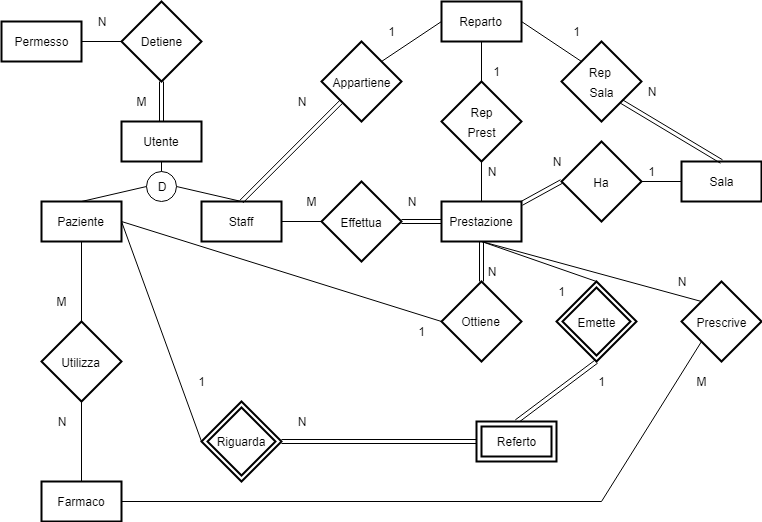
\includegraphics[scale=0.8]{Diagramma}
%\end{figure}

\begin{center}
\vspace{0.5cm}
\begin{tikzpicture}[
	%->, frecce orietate
	%>=stealth',
  %	%shorten >=1pt,
  	auto,	
  	semithick, %linee più spesse
	node distance=7em,
	scale=0.8, transform shape] 
	
	\node[relationship] (detiene) [above=of utente] {Detiene};
	\node[entity] (ruolo) [left = 1cm of detiene] {Ruolo} edge node{1} (detiene);
	\node[entity] (utente) {Utente} edge [total] node {N} (detiene);
	\node[isa] (isa) [below of = utente] {d} edge [total] (utente);	
	\node[entity] (staff) [below right = 2cm of isa] {Staff} edge (isa);
	\node[entity] (paziente) [below left = 2cm of isa] {Paziente} edge (isa);
	\node[relationship] (utilizza) [below=of paziente] {Utilizza} edge node{M} (paziente);
	\node[entity] (farmaco) [below of = utilizza] {Farmaco} edge node{N} (utilizza);
	
	\node[relationship] (effettua) [right=of staff] {Effettua} edge node{M} (staff);
	\node[entity] (prestazione) [right = 1cm of effettua] {Prestazione} edge [total] node{N} (effettua);
	
	\node[relationship] (ottiene) [below=of prestazione] {Ottiene} edge [total] node{N} (prestazione);
	\path (ottiene) edge node{1} (paziente);
	
	\node[ident relationship] (emette) [below right=of prestazione] {Emette} edge node{1} (prestazione);
	\node[weak entity] (referto) [below left=3cm of emette] {Referto};
	\path (emette) edge [total] node{1} (referto);
	\node[ident relationship] (riguarda) [left=of referto] {Riguarda} edge [total] node{N} (referto);
	\path (paziente) edge node{1} (riguarda);
	
	\node[relationship] (prescrive) [below left= 3.5cm of prestazione] {Prescrive} edge node{N} (prestazione);
	\path (prescrive) edge node{M} (farmaco);
	
	\node[relationship] (rep_pres) [above= of prestazione] {Rep Prest} edge [total] node{N} (prestazione);
	\node[entity] (reparto) [above=of rep_pres] {Reparto} edge node{1} (rep_pres);
	
	\node[relationship] (appartiene) [above right= of staff] {Appartiene} edge [total] node{N} (staff);
	\path (appartiene) edge node{1} (reparto);
	
	
	\node[relationship] (ha) [above right= of prestazione] {Ha};
	\node[entity] (sala) [right=of ha] {Sala};
	\path (ha) edge node{1} (sala);
	\path (ha) edge [total] node{N} (prestazione);
	
	\node[relationship] (rep_sala) [above left= of sala] {Rep Sala} edge node{1} (reparto);
	\path (rep_sala) edge [total] node{N} (sala);
	
			
\end{tikzpicture}
\vspace{0.5cm}
\end{center}



%%%%%%%%%%%%%%%%%%%%%%%%%%% Da Modello ER a Modello Relazionale
\chapter{Da Modello ER a Modello Relazionale}
Dopo aver completato lo schema ER, è necessario mappare le entità e le relazioni sul database. Questa procedura avviene secondo i seguenti passi:

\begin{itemize}
\item Traduzione di tipi di entità
\begin{itemize}
\item Traduzione entità forti.
\item Traduzione entità deboli e specializzazioni.
\end{itemize}
\item Traduzione di tipi di associazioni binarie.
\begin{itemize}
\item Traduzioni associazioni 1:1.
\item Traduzione associazioni 1:N.
\item Traduzione associazioni N:M.
\end{itemize} 
\item Traduzione di attributi multivalore.
\item Traduzioni di tipi di associazione N-arie.
\end{itemize}

\section{Traduzione entità forti}
Per ogni tipo di entità forte E nello schema ER, viene costruita una relazione R che contiene tutti gli attributi semplice di E. Di un attributo composto vanno inseriti solamente gli attributi componenti semplici. Come chiave primaria viene scelto uno degli attributi chiavi di E.
Le entità forti presenti nello schema sono:
\begin{itemize}
\item Utente
\item Farmaco
\item Reparto
\item Sala
\item Prestazione
\item Ruolo
\end{itemize}
Le chiavi primarie sono evidenziate in giallo, le chiavi esterne in verde e gli attributi unici in azzurro. La loro rappresentazione è la seguente:
\begin{figure}[H]
\begin{center}
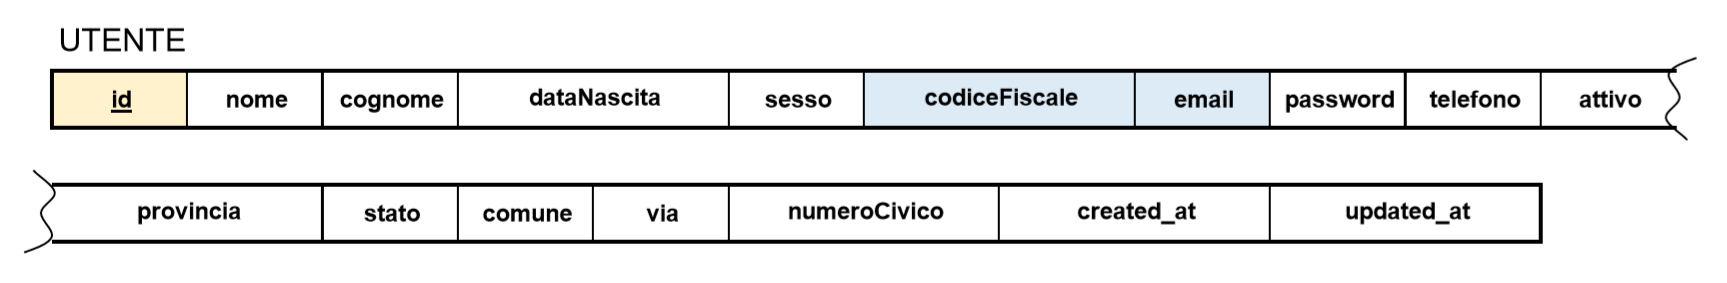
\includegraphics[scale=0.3]{utenteSchema}
\end{center}
\end{figure}

\begin{figure}[H]
\begin{center}
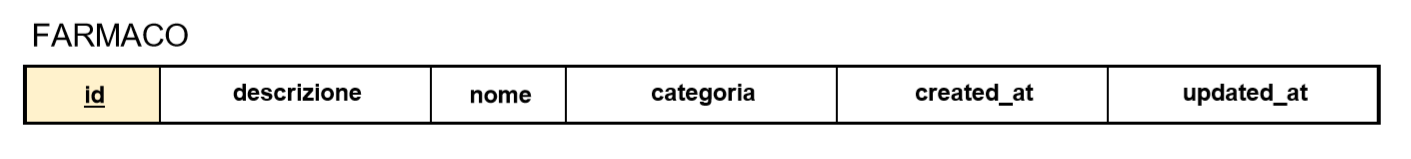
\includegraphics[scale=0.3]{farmacoSchema}
\end{center}
\end{figure}

\begin{figure}[H]
\begin{center}
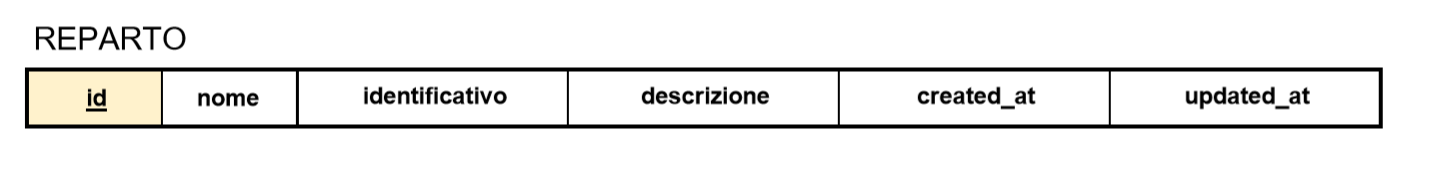
\includegraphics[scale=0.3]{repartoSchema}
\end{center}
\end{figure}

\begin{figure}[H]
\begin{center}
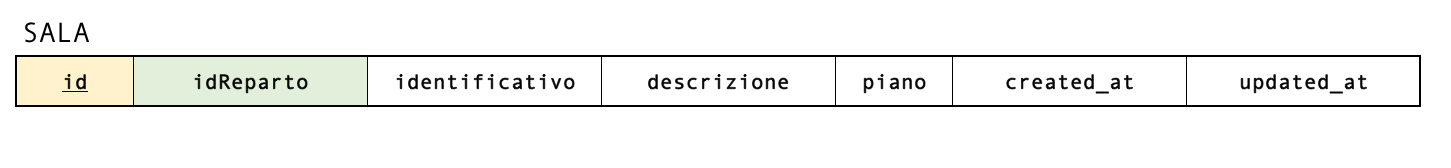
\includegraphics[scale=0.3]{salaSchema}
\end{center}
\end{figure}

\begin{figure}[H]
\begin{center}
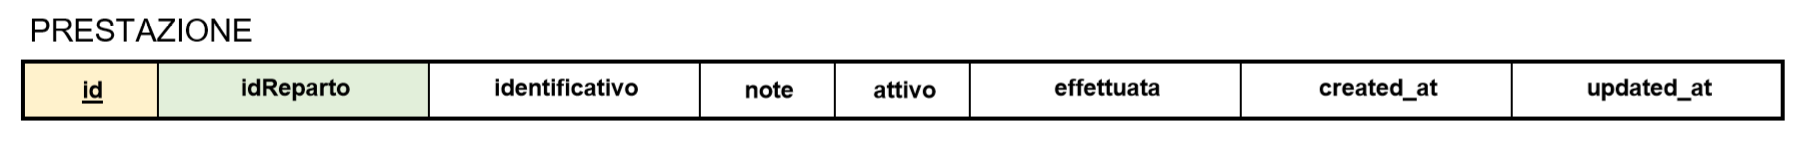
\includegraphics[scale=0.26]{prestazioneSchema}
\end{center}
\end{figure}

\begin{figure}[H]
\begin{center}
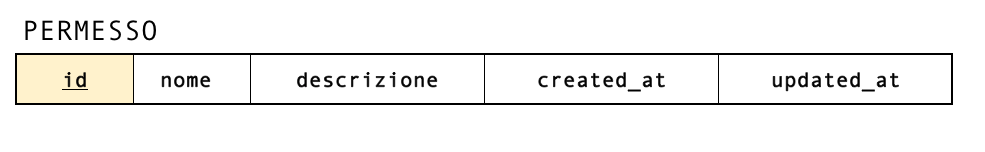
\includegraphics[scale=0.3]{permessiSchema}
\end{center}
\end{figure}

\section{Traduzione entità deboli e specializzazioni}
Per ogni tipo di entità debole W dello scema ER con entità proprietaria E, viene costruita una relazione R che ha come attributi, tutti gli attributi semplici di W. Inoltre vengono inseriti come attributi di chiave esterna in R, le chiavi primarie delle relazioni proprietari. La chiave primaria di R è data dalla combinazione della chiave primaria delle varie entità proprietarie e dell'eventuale chiave parziale dell'entità debole W.
Nello schema è presente un'unica entità debole: \textit{Referto}
\begin{figure}[H]
\begin{center}
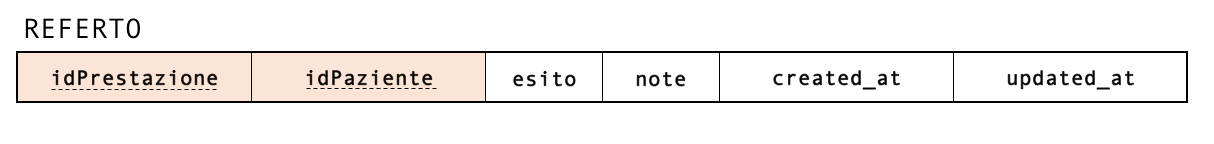
\includegraphics[scale=0.3]{refertoSchema}
\end{center}
\end{figure}
Gli attributi \textit{idPrestazione} e \textit{idPaziente} sono rispettivamente le chiavi primarie di \textit{Prestazione} e \textit{Paziente}, entità proprietarie di \textit{Referto}. La chiave primaria di \textit{Referto} è quindi la combinazione di \textit{idPrestazione} e \textit{idPaziente} (\textit{Referto} non ha chiave parziale).\\

Le specializzazioni di \textit{Utente} (\textit{Paziente} e \textit{Staff}) sono rappresentate nel modo seguente:
\begin{figure}[H]
\begin{center}
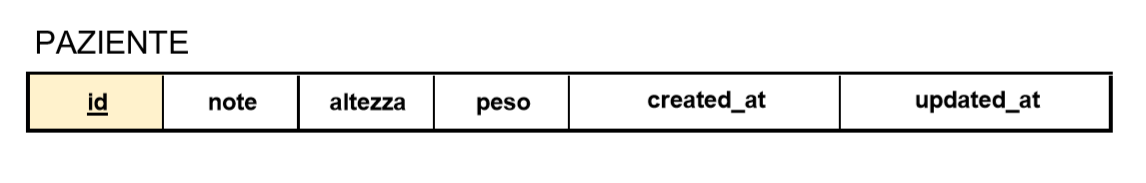
\includegraphics[scale=0.3]{pazienteSchema}
\end{center}
\end{figure}

\begin{figure}[H]
\begin{center}
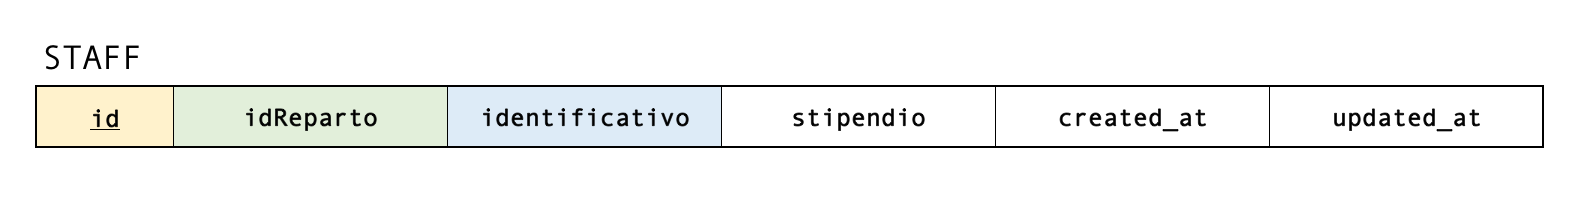
\includegraphics[scale=0.3]{staffSchema}
\end{center}
\end{figure}

dove \textit{id} rappresenta, sia per \textit{Paziente} che per \textit{Staff}, l'identificativo dell'utente (chiave primaria della tabella \textit{Utente}). In \textit{Staff} è stata anche inserita, come chiave esterna (a causa della relazione \textit{N:1} che lega \textit{Staff} a \textit{Reparto}) la chiave primaria di \textit{Reparto} (i.e. \textit{idReparto}). 

\section{Traduzioni associazioni 1:1}
L'unica relazione \textit{1:1} è \textit{Emette}, che collega \textit{Prestazione} a \textit{Referto}. Essendo \textit{Referto} una entità debole collegata a \textit{Prestazione}, in \textit{Referto} viene inserita la chiave primaria di \textit{Referto}. 

\section{Traduzioni associazioni 1:N}
Per ogni associazione R binaria del tipo \textit{1:N} nello schema ER, vengono individuate le due relazioni corrispondenti alle due entità partecipanti. Viene quindi inserita nel lato \textit{N}, la chiave primaria della relazione lato \textit{1}. In questo caso sono quindi state inserite le seguenti chiavi:
\begin{itemize}
\item \textit{id} di \textit{Paziente} in \textit{Referto}.
\item \textit{id} di \textit{Paziente} in \textit{Prestazione}.
\item \textit{id} di \textit{Reparto} in \textit{Staff}.
\item \textit{id} di \textit{Reparto} in \textit{Sala}.
\item \textit{id} di \textit{Sala} in \textit{Prestazione}.
\end{itemize}

\section{Traduzioni associazioni N:M}
Per ogni associazione binaria R del tipo \textit{N:M}, viene costruita una nuova relazione S che la rappresenta. Come attributi di chiave esterna si S, vengono inserite le chiavi primarie delle relazioni rappresentanti le entità partecipanti: la combinazione di queste due chiavi forma la chiave primaria di S. In particolare:

\begin{itemize}
\item StaffPrestazione: contiene, come chiavi esterne, le chiavi primarie delle tabelle \textit{Staff} e \textit{Prestazione}.
\item PazienteFarmaco: contiene, come chiavi esterne, le chiavi primarie delle tabelle \textit{Paziente} e \textit{Farmaco}.
\item PrestazioneFarmaco: contiene, come chiavi esterne, le chiavi primarie delle tabelle \textit{Prestazione} e \textit{Farmaco}.
\item RuoloUtente: contiene, come chiavi esterne, le chiavi primarie delle tabelle \textit{Ruolo} e \textit{Utente}.
\end{itemize}

\begin{figure}[H]
\begin{center}
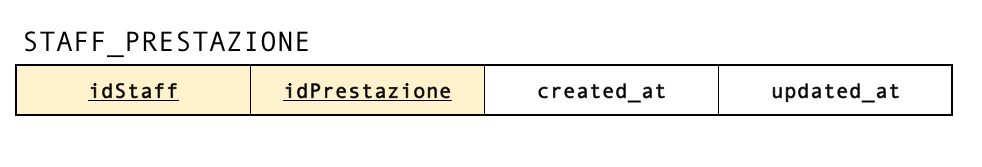
\includegraphics[scale=0.3]{staffPrestazioneSchema}
\end{center}
\end{figure}

\begin{figure}[H]
\begin{center}
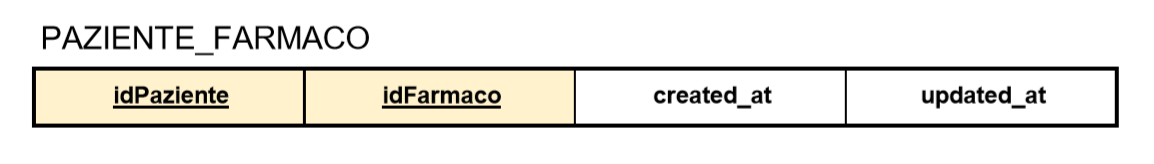
\includegraphics[scale=0.3]{pazienteFarmacoSchema}
\end{center}
\end{figure}

\begin{figure}[H]
\begin{center}
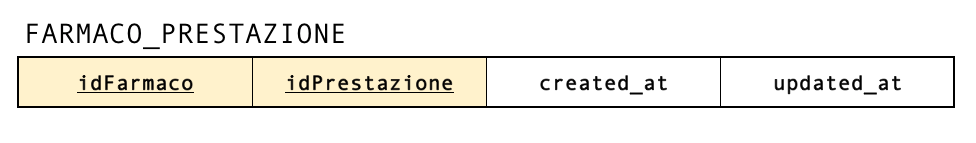
\includegraphics[scale=0.3]{farmacoPrestazioneSchema}
\end{center}
\end{figure}

\begin{figure}[H]
\begin{center}
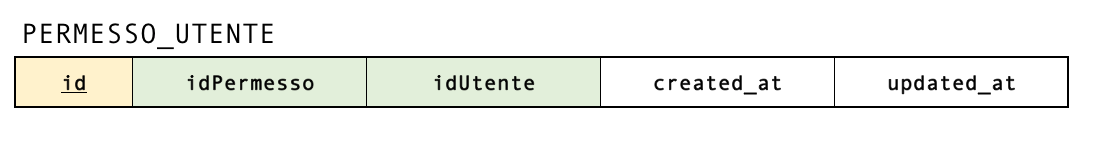
\includegraphics[scale=0.3]{permessiUtenteSchema}
\end{center}
\end{figure}

Per ogni associazione \textit{N:M} viene quindi creata una nuova tabella nel database.

%%%%%%%%%%%%%%%%%%%%%%%%%%%%%%%%%%%%%%
\chapter{Normalizzazione}
Il processo di normalizzazione si basa su una serie di test che verificano se uno schema di relazione soddisfa una determinata \textit{forma normale}. Esistono diversi tipi di forma normale:
\begin{itemize}
\item Prima forma normale (1NF).
\item Seconda forma normale (2NF).
\item Terza forma normale (3NF).
\item Forma normale di Boyce e Codd.
\item Quarta forma normale (4NF).
\item Quinta forma normale.
\end{itemize}
L'obiettivo della normalizzazione dei dati è quello di minimizzare la ridondanza e le anomalie dovute all'inserimento, cancellazione o modifica dei dati nel database. Questa caratteristica si ottiene attraverso una analisi degli schemi forniti e una decomposizione degli schemi che non soddisfano certe condizioni, in schemi più piccoli (che verificano le proprietà desiderate). In questa applicazione, si raggiunge solamente la terza forma normale.
\\
La \textit{prima forma normale} richiede che il dominio di un attributo contenga solamente valori indivisibili e che il valore di un qualsiasi attributo in una tupla sia un valore singolo del dominio. Lo schema presentato è già in prima forma normale.
\\
Per soddisfare la \textit{seconda forma normale}, nello schema di relazione R, ogni attributo non primo di R (quindi non fa parte di una chiave candidata) deve dipendete funzionalmente in modo completo dalla chiave primaria di R. La definizione di dipendenza funzionale completa è le seguente: una dipendenza funzionale $X \rightarrow Y$ si dice \textit{dipendenza funzionale completa} se la rimozione di un qualsiasi attributo A da X, comporta che la dipendenza funzionale non sussista più. Per ottenere la seconda forma normale, si decompone la relazione principale R in un certo numero di relazioni nelle quali gli attributi non primi sono associati solamente alla parte della chiave primaria da cui sono funzionalmente dipendenti in modo completo. Lo schema soddisfa anche la seconda forma normale.
\\
Uno schema di relazione R è in \textit{terza forma normale} se soddisfa la seconda forma normale e nessun attributo non primo di R dipende in modo transitivo dalla chiave primaria. Lo schema presentato, come per i casi precedenti, soddisfa anche la terza forma normale senza bisogno di ulteriori modifiche.

\begin{figure}
\begin{center}
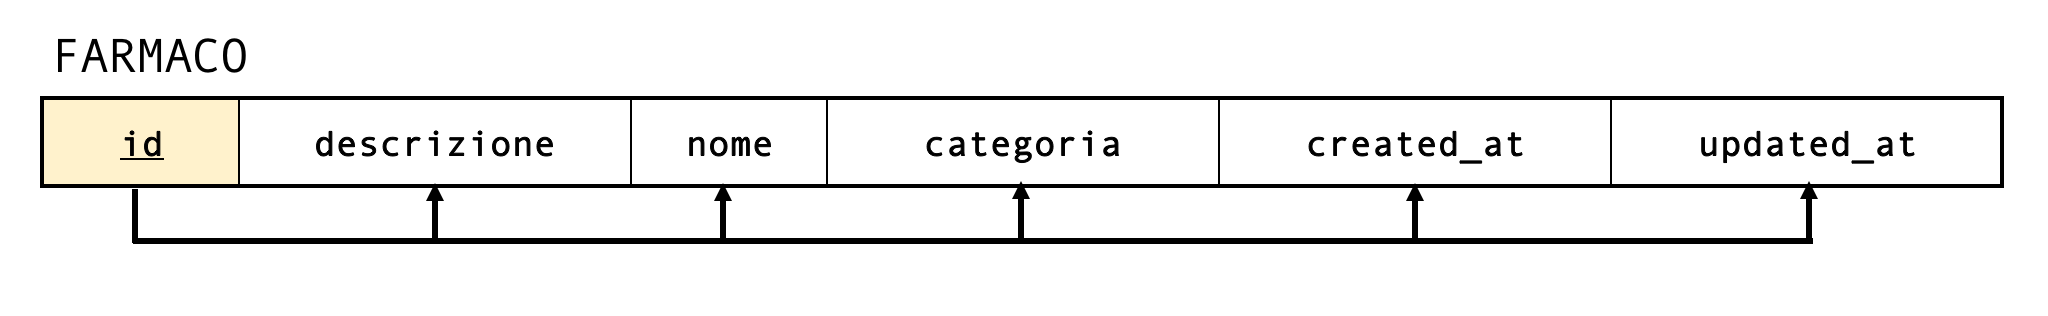
\includegraphics[scale=0.35]{immagini_normalizzazione/farmaco}
\end{center}
\end{figure}

\begin{figure}[H]
\begin{center}
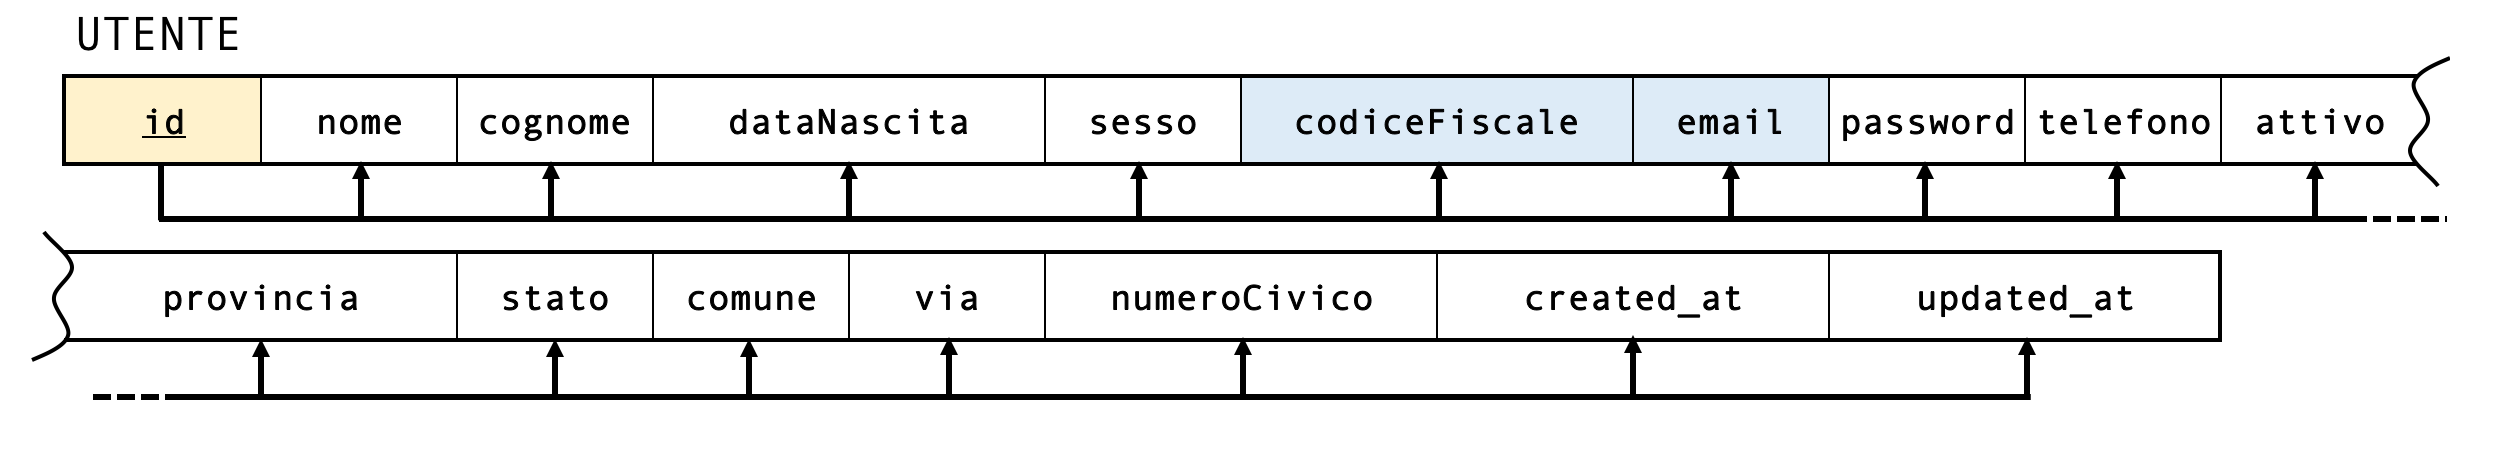
\includegraphics[scale=0.35]{immagini_normalizzazione/utente}
\end{center}
\end{figure}

\begin{figure}[H]
\begin{center}
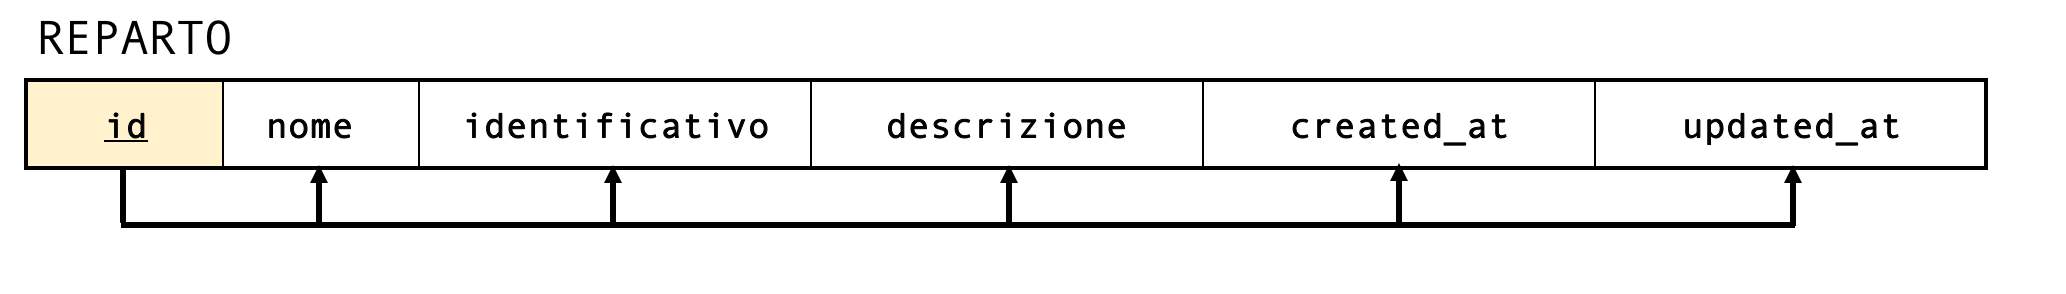
\includegraphics[scale=0.35]{immagini_normalizzazione/reparto}
\end{center}
\end{figure}

\begin{figure}[H]
\begin{center}
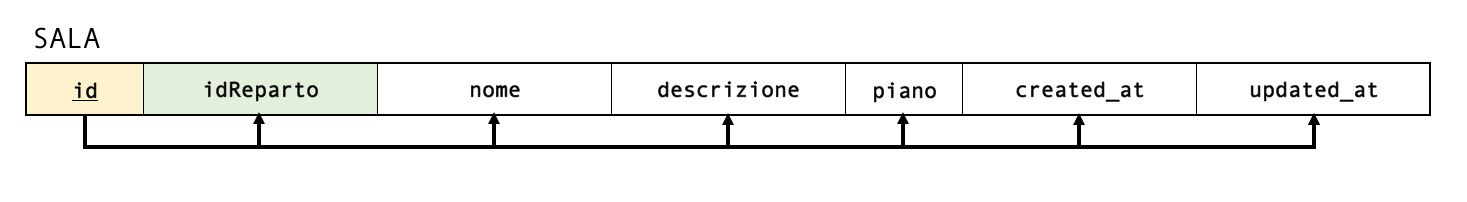
\includegraphics[scale=0.35]{immagini_normalizzazione/sala}
\end{center}
\end{figure}

\begin{figure}[H]
\begin{center}
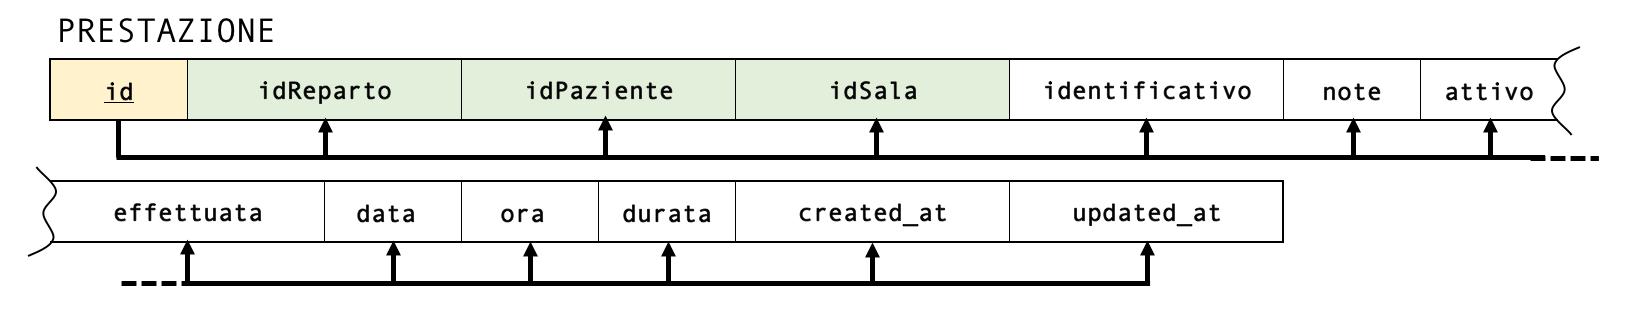
\includegraphics[scale=0.25]{immagini_normalizzazione/prestazione}
\end{center}
\end{figure}

\begin{figure}[H]
\begin{center}
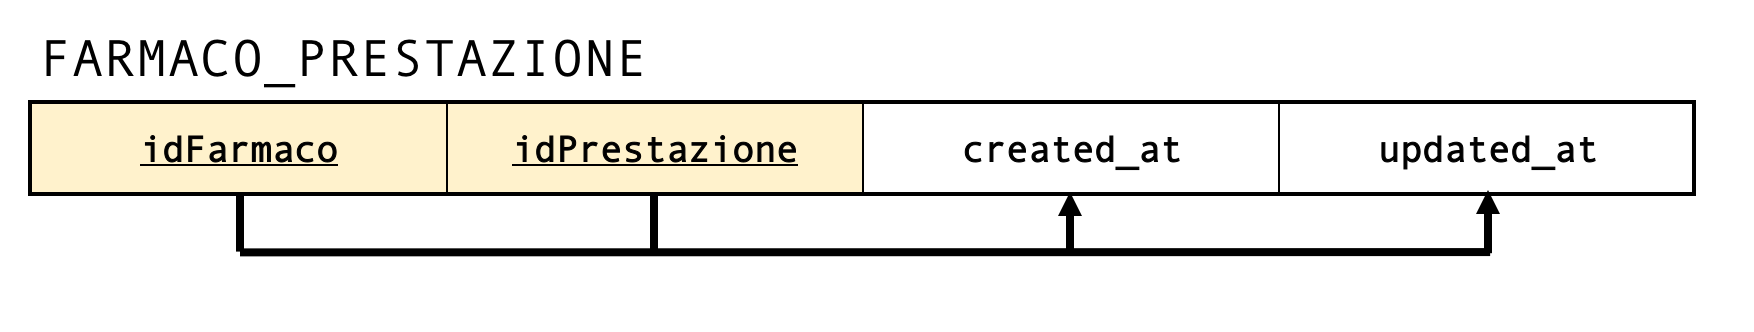
\includegraphics[scale=0.35]{immagini_normalizzazione/farmaco_prestazione}
\end{center}
\end{figure}

\begin{figure}[H]
\begin{center}
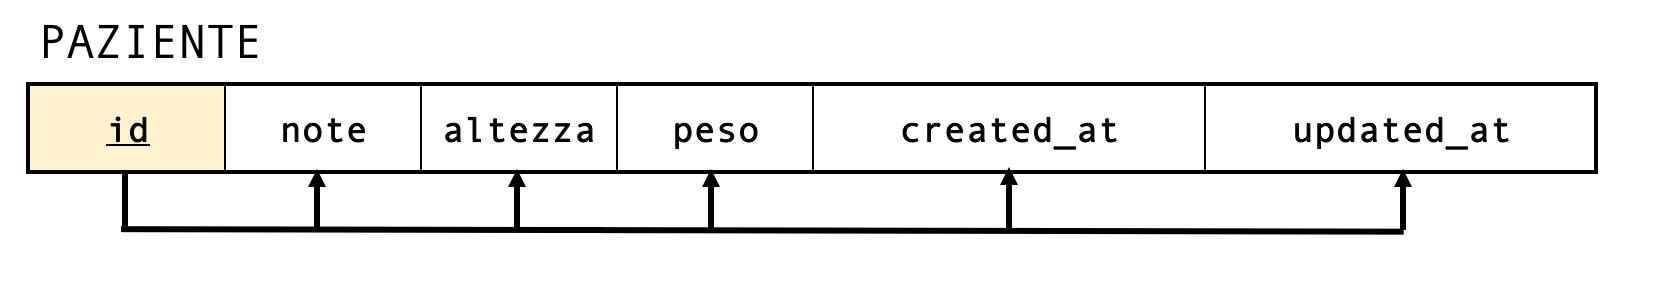
\includegraphics[scale=0.35]{immagini_normalizzazione/paziente}
\end{center}
\end{figure}

\begin{figure}[H]
\begin{center}
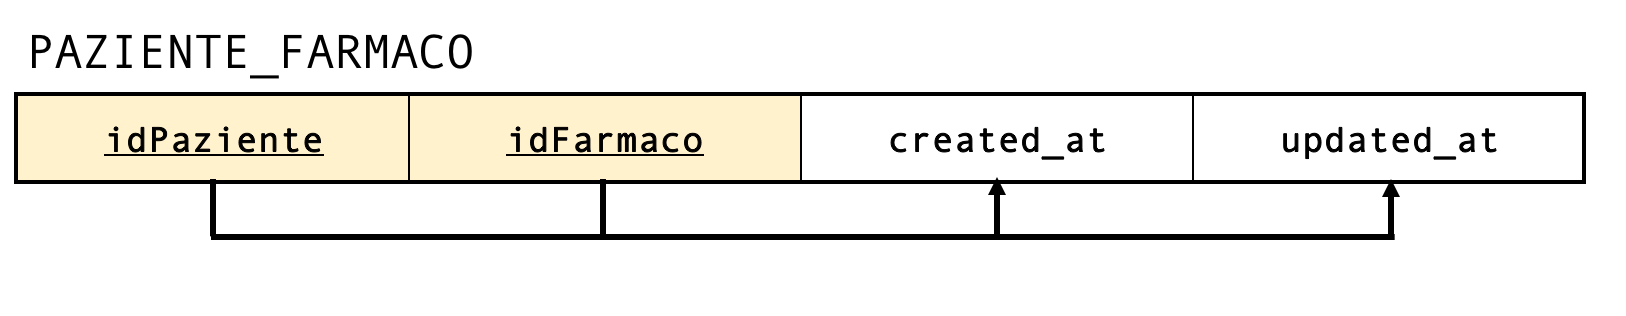
\includegraphics[scale=0.35]{immagini_normalizzazione/paziente_farmaco}
\end{center}
\end{figure}

\begin{figure}[H]
\begin{center}
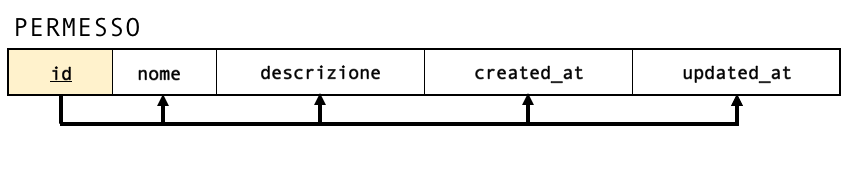
\includegraphics[scale=0.35]{immagini_normalizzazione/permessi}
\end{center}
\end{figure}

\begin{figure}[H]
\begin{center}
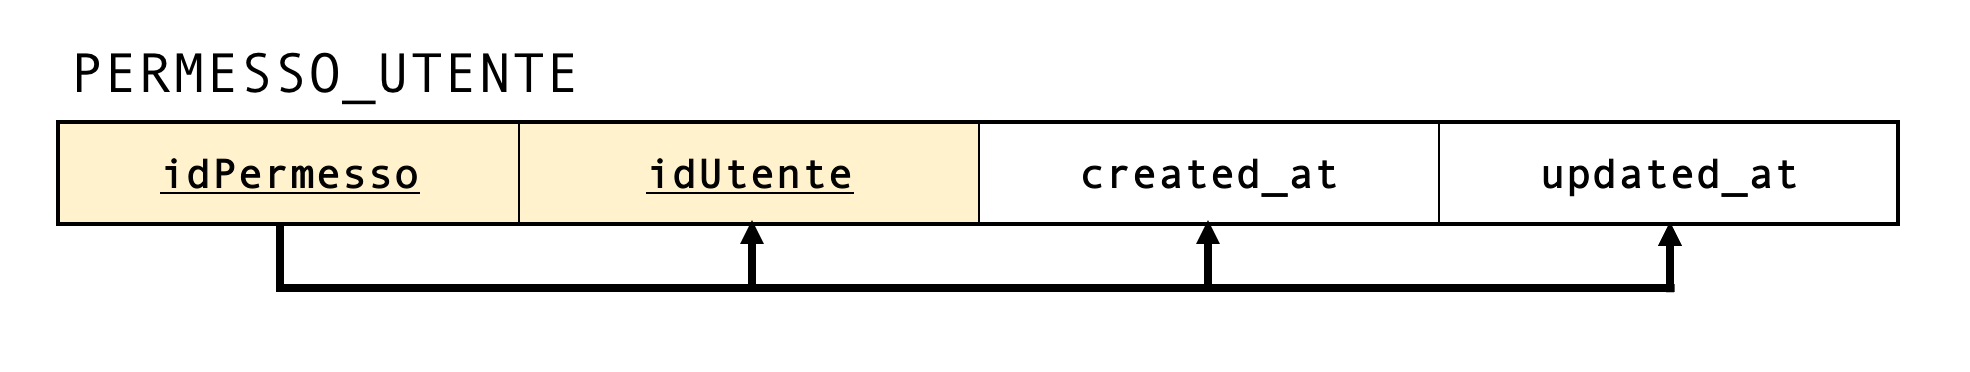
\includegraphics[scale=0.33]{immagini_normalizzazione/permessi_utente}
\end{center}
\end{figure}

\begin{figure}[H]
\begin{center}
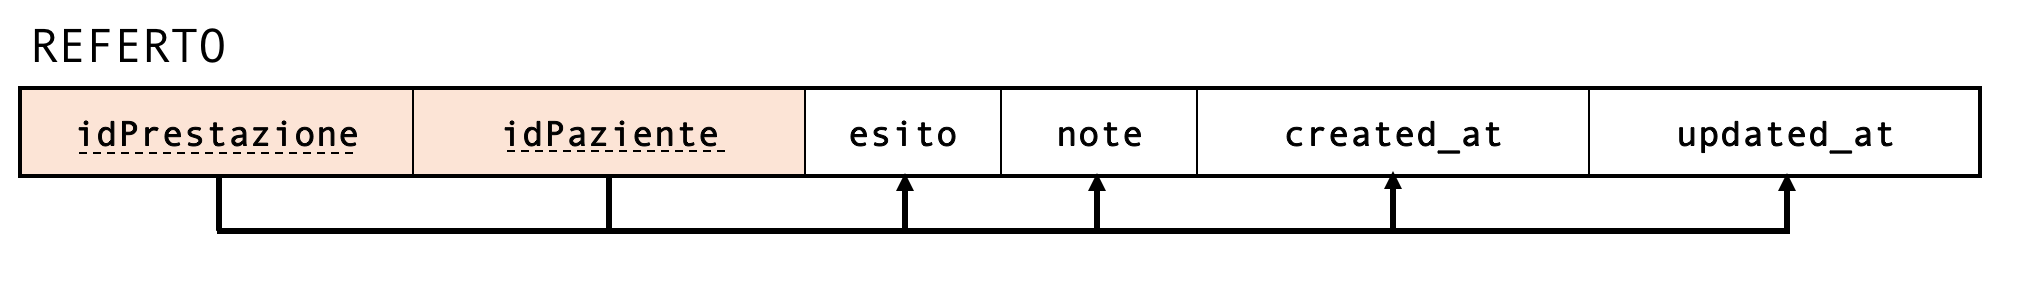
\includegraphics[scale=0.35]{immagini_normalizzazione/referto}
\end{center}
\end{figure}

\begin{figure}[H]
\begin{center}
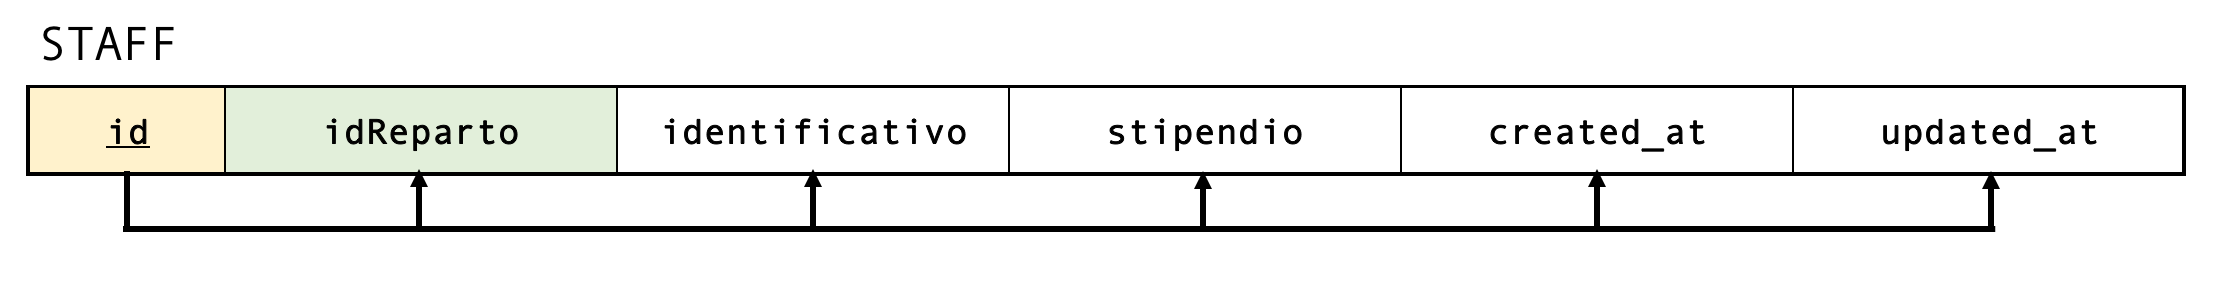
\includegraphics[scale=0.35]{immagini_normalizzazione/staff}
\end{center}
\end{figure}

\begin{figure}[H]
\begin{center}
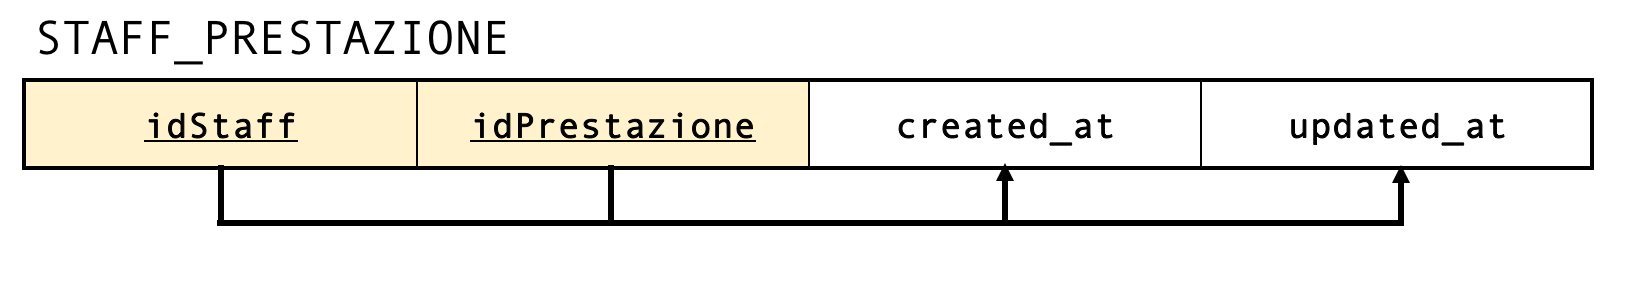
\includegraphics[scale=0.35]{immagini_normalizzazione/staff_prestazione}
\end{center}
\end{figure}

Di seguito lo schema completo in \textit{terza forma normale}.
\begin{figure}
\begin{center}
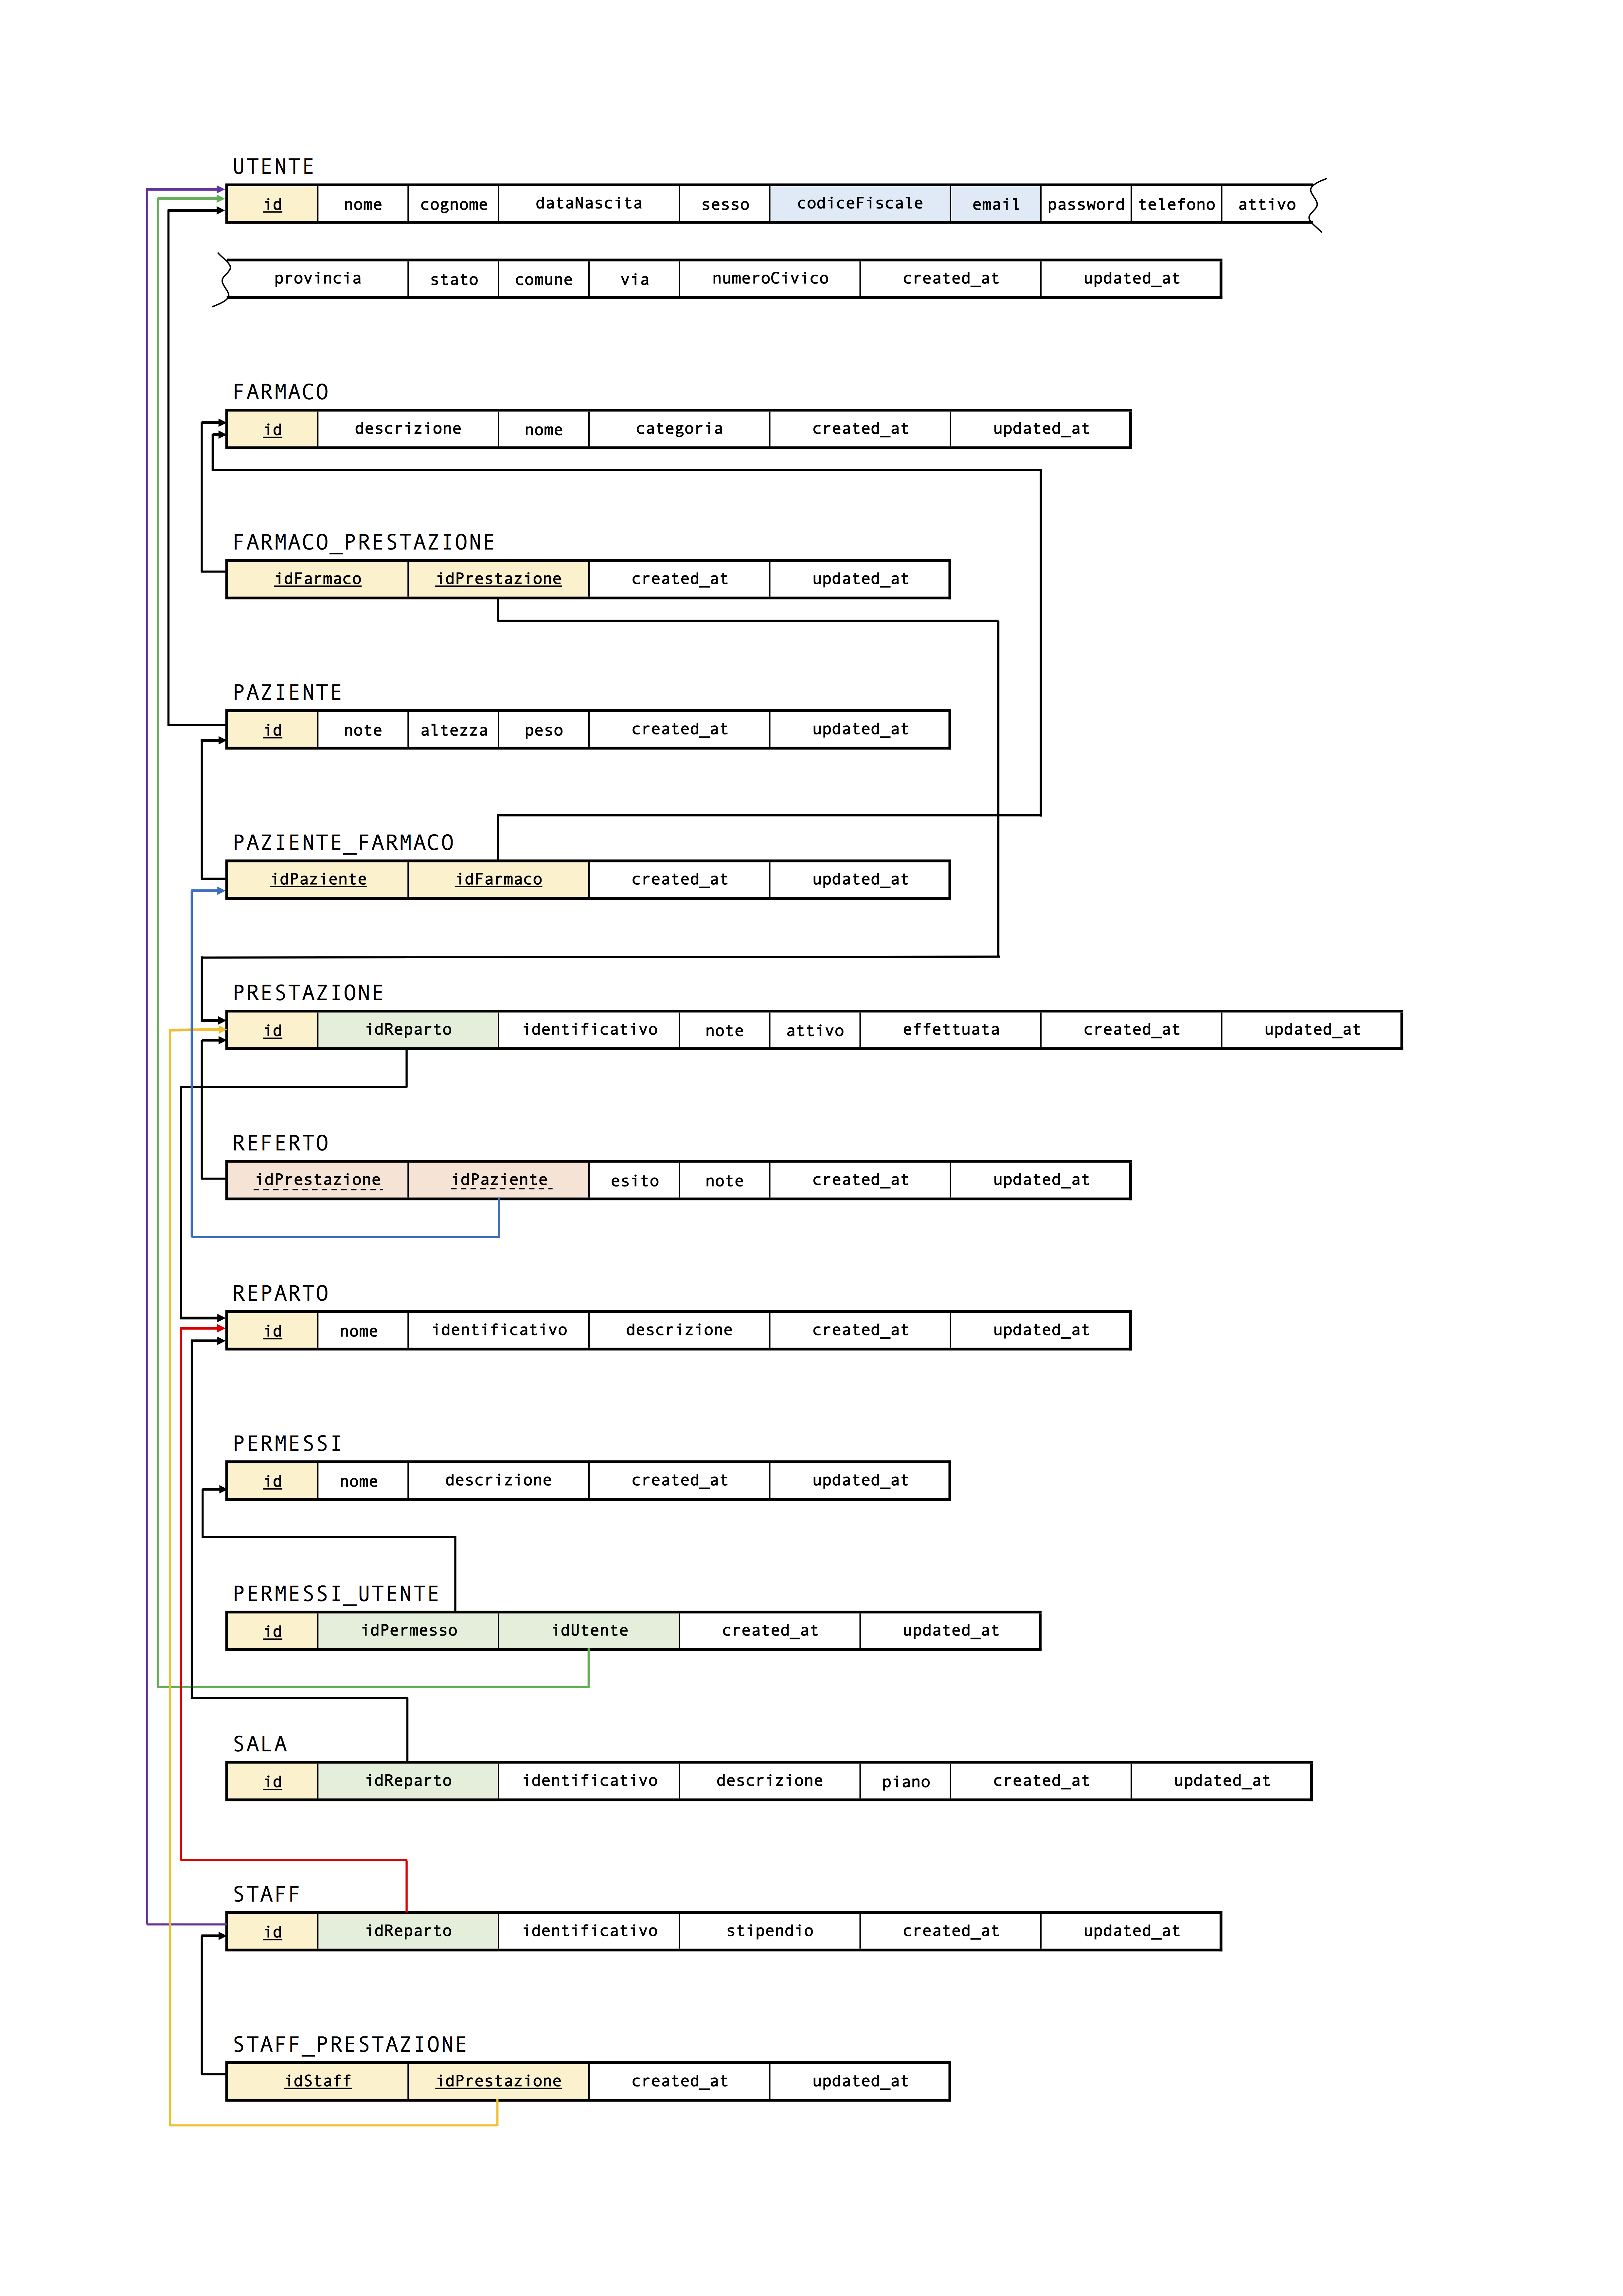
\includegraphics[scale=0.85]{schema_relazionale}
\end{center}
\end{figure}

%%%%%%%%%%%%%%%%%%%%%%%%%%% NORMALIZZAZIONE


%%%%%%%%%%%%%%%%%%%%%%%%%%% CODICE SQL
\chapter{Codice SQL}
\section{Introduzione}
L'intero progetto è stato sviluppato utilizzando il framework php \textit{Laravel}. Le tabelle del database sono state create utilizzando le \texttt{migration}. Per ogni tabella del database è stato eseguito il comando \texttt{php artisan make:migration create\_table\_nomeTabella}. Questo comando genera una classe \texttt{migration} all'interno del file \texttt{create\_table\_nomeTabella.php} nella quale sono definiti i metodi \texttt{up()} e \texttt{down()}. All'interno di \texttt{up()} vengono inseriti tutti i comandi per la creazione delle tabelle. Generate le migrations per tutte le tabelle, il comando \texttt{php artisan migrate} traduce i comandi specificati nel metodo \texttt{up}, in comandi SQL per la creazione delle tabelle. Di seguito viene riportato il codice SQL generato dalle migrations.
\section{Codice Creazione Tabelle}
\begin{verbatim}
UTENTE
CREATE TABLE utente (
        id INT AUTO_INCREMENT PRIMARY_KEY,
        nome VARCHAR(255) NOT NULL,
        cognome VARCHAR(255) NOT NULL,
        dataNascita DATE NOT NULL,
        sesso BIT NOT NULL,
        codiceFiscale VARCHAR(255) NOT NULL UNIQUE, 
        email VARCHAR(255) NOT NULL UNIQUE,
        password VARCHAR(255) NOT NULL,
        telefono VARCHAR(255) NOT NULL,
        attivo BIT NOT NULL,
        provincia VARCHAR(255) NOT NULL,
        stato VARCHAR(255) NOT NULL,
        comune VARCHAR(255) NOT NULL,
        via VARCHAR(255) NOT NULL,
        numeroCivico INT NOT NULL,
        timestamp TIMESTAMP         
);

PAZIENTE
CREATE TABLE paziente (
        id INT FOREGIN_KEY REFERENCES utente(id),
        note TEXT,
        altezza INT NOT NULL,
        peso INT NOT NULL,
        timestamp TIMESTAMP        
);

REPARTO
CREATE TABLE reparto (
	    id INT PRIMARY_KEY,
        nome VARCHAR(255) NOT_NULL, 
        identificativo VARCHAR(255) NOT NULL,
        descrizione TEXT,
        timestamp TIMESTAMP, 
);

SALA
CRATE TABLE sala (
        id INT AUTO INCREMENT PRIMARY KEY,
        identificativo VARCHAR(255) NOT NULL,
        idReparto INT FOREGIN KEY REFERENCES reparto(id),
        piano INT,
       	timestamp TIMESTAMP
);

STAFF
CREATE TABLE staff (
        id INT FOREGIN_KEY REFERENCES utente(id),
        idReparto INT FOREGIN_KEY REFERENCES reparto(id),
        identificativo VARCHAR(255) NOT NULL,
        contenuto TETX NOT_NULL,
        timestamp TIMESTAMP
);

FARMACO
CREATE TABLE farmaco (
        id INT AUTO INCREMENT PRIMARY KEY,
        descrizione TEXT NOT NULL,
        nome VARCHAR(255) NOT NULL,
        categoria VARCHAR(255) NOT NULL,
       	timestamp TIMESTAMP
);

PRESTAZIONE
CREATE TABLE prestazione (
        id INT AUTO_INCREMENT PRIMARY_KEY,
        idReparto INT FOREGIN_KEY REFERENCES reparto(id),
        idSala INT FOREGIN_KEY REFERENCES sala(id),
        identificativo VARCHAR(255) NOT NULL,
        note TEXT,
        attivo BIT NOT NULL,
        effettuata BIT NOT NULL,
        timestamp TIMESTAMP
);

REFERTO
CREATE TABLE referto (
        id INT FOREGIN_KEY REFERENCES prestazione(id),
        idPaziente INT FOREGIN_KEY REFERENCES prestazione(idPaziente),
        identificativo VARCHAR(255) NOT NULL,
        esito TEXT NOT NULL,
        note TEXT,
        timestamp TIMESTAMP
);

STAFF_PRESTAZIONE
CREATE TABLE staff_prestazione (
        idPrestazione INT FOREGIN_KEY REFERENCES prestazione(id),
        idStaff INT FOREGIN_KEY REFERENCES staff(id),
        timestamp TIMESTAMP
);

PAZIENTE_FARMACO
CREATE TABLE paziente_farmaco (
        idPaziente INT FOREGIN_KEY REFERENCES paziente(id),
        idFarmaco INT FOREGIN_KEY REFERENCES farmaco(id),
        timestamp TIMESTAMP
);

FARMACO_PRESTAZIONE
CREATE TABLE farmaco_prestazione (
        idPrestazione INT FOREGIN_KEY REFERENCES prestazione(id),
        idFarmaco INT FOREGIN_KEY REFERENCES farmaco(id),
        timestamp TIMESTAMP
);

UTENTE_ROLE
CREATE TABLE utente_role (
        user_id INT FOREGIN_KEY REFERENCES utente(id),
        role_id INT FOREGIN_KEY REFERENCES role(id),
        timestamp TIMESTAMP
);

ROLES
CREATE TABLE roles (
        id INT PRIMARY_KEY,
        name VARCHAR(255) NOT NULL,
        description TEXT,
        timestamp TIMESTAMP
);
\end{verbatim}

%%%%%%%%%%%%%%%%%%%%%%%%%%% INTERROGAZIONI
\chapter{Query}
Di seguito vengono riportate alcune query significative utilizzate nell'applicazione.
\begin{itemize}
\item Ricavare il nome di un farmaco utilizzato in una prestazione (identificata da \$id):
\begin{verbatim}
SELECT nome
FROM farmaco
JOIN farmaco_prestazione ON farmaco_prestazione.idFarmaco = farmaco.id
WHERE farmaco_prestazione.id = $idPrestazione 
\end{verbatim}

\item Aggiornamento dati paziente (identificato da \$id):
\begin{verbatim}
UPDATE paziente
SET peso = $peso, altezza = $altezza, note = $note
WHERE id = $id 
\end{verbatim}

\item Eliminazione di un reparto (identificato da \$id):
\begin{verbatim}
DELETE FROM reparto
WHERE id = $id 
\end{verbatim}

\item Ricerca di un componente dello staff (identificato da \$id) dati nome e cognome incompleti (utilizzato per l'autocompletamento):
\begin{verbatim}
SELECT utente.id, utente.nome, utente.cognome, 
        staff.identificativo as identificativoPersonale, 
        staff.idReparto as idReparto,
        reparto.identificativo as identificativoReparto 
FROM utente
JOIN staff ON utente.id = staff.id
JOIN reparto ON reparto.id = staff.idReparto
WHERE utente.attivo = '1' AND
            (CONCAT(utente.nome, ' ', utente.cognome) LIKE '$search%' OR 
            CONCAT(utente.cognome, ' ', utente.nome) LIKE '$search%')
\end{verbatim}

\item Inserimento di una sala relativa al reparto di Cardiologia:
\begin{verbatim}
INSERT INTO sala 
SET 
	nome = 'Sala1', 
	descrizione = 'Nuova sala', 
	piano = '2', 
    id_reparto = (
    	SELECT id
        FROM reparto,
        WHERE name = 'Cardiologia')
\end{verbatim}

\end{itemize}

%%%%%%%%%%%%%%%%%%%%%%%%%%% INTERFACCIA
\chapter{Interfaccia}

\begin{figure}[H]
\begin{center}
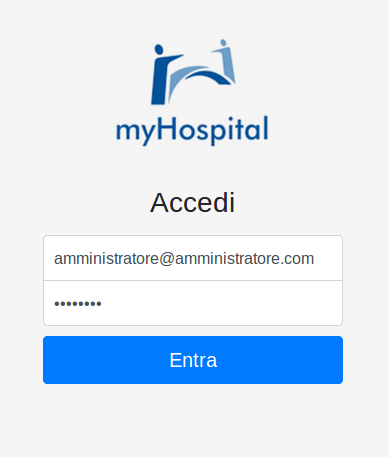
\includegraphics[scale=1]{grafica/Login}
\caption{Schermata di Login.}
\end{center}
\end{figure}

\begin{landscape}
\begin{figure}[H]
\begin{center}
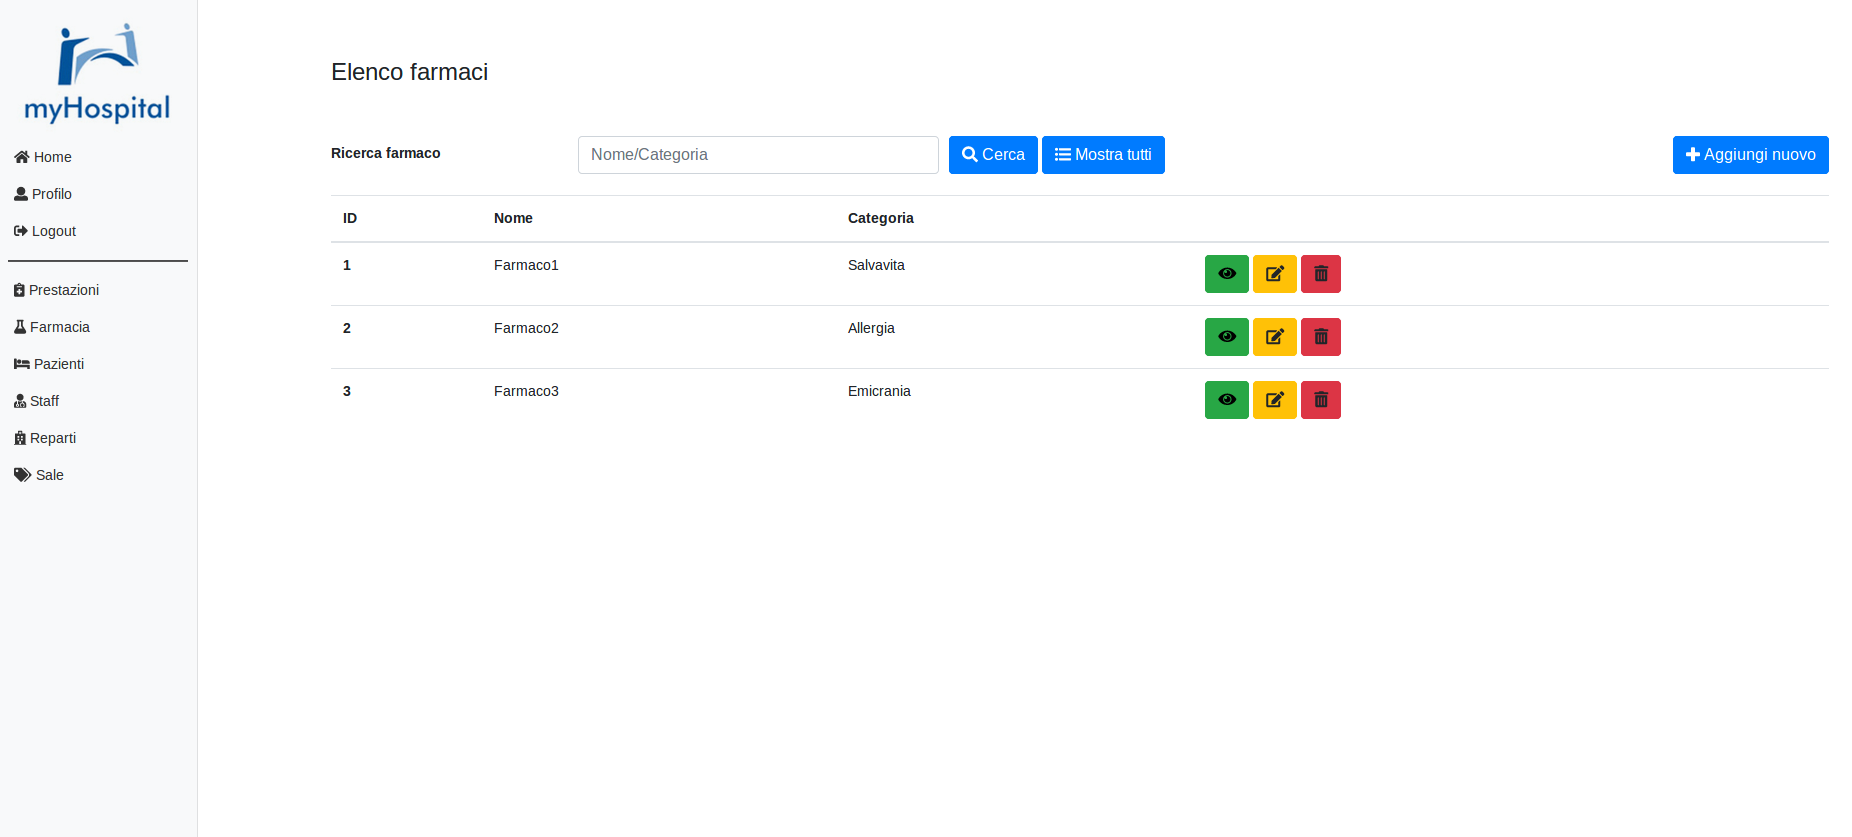
\includegraphics[scale=0.6]{grafica/ElencoFarmaci}
\caption{Elenco dei farmaci.}
\end{center}
\end{figure}
\end{landscape}

\begin{landscape}
\begin{figure}[H]
\begin{center}
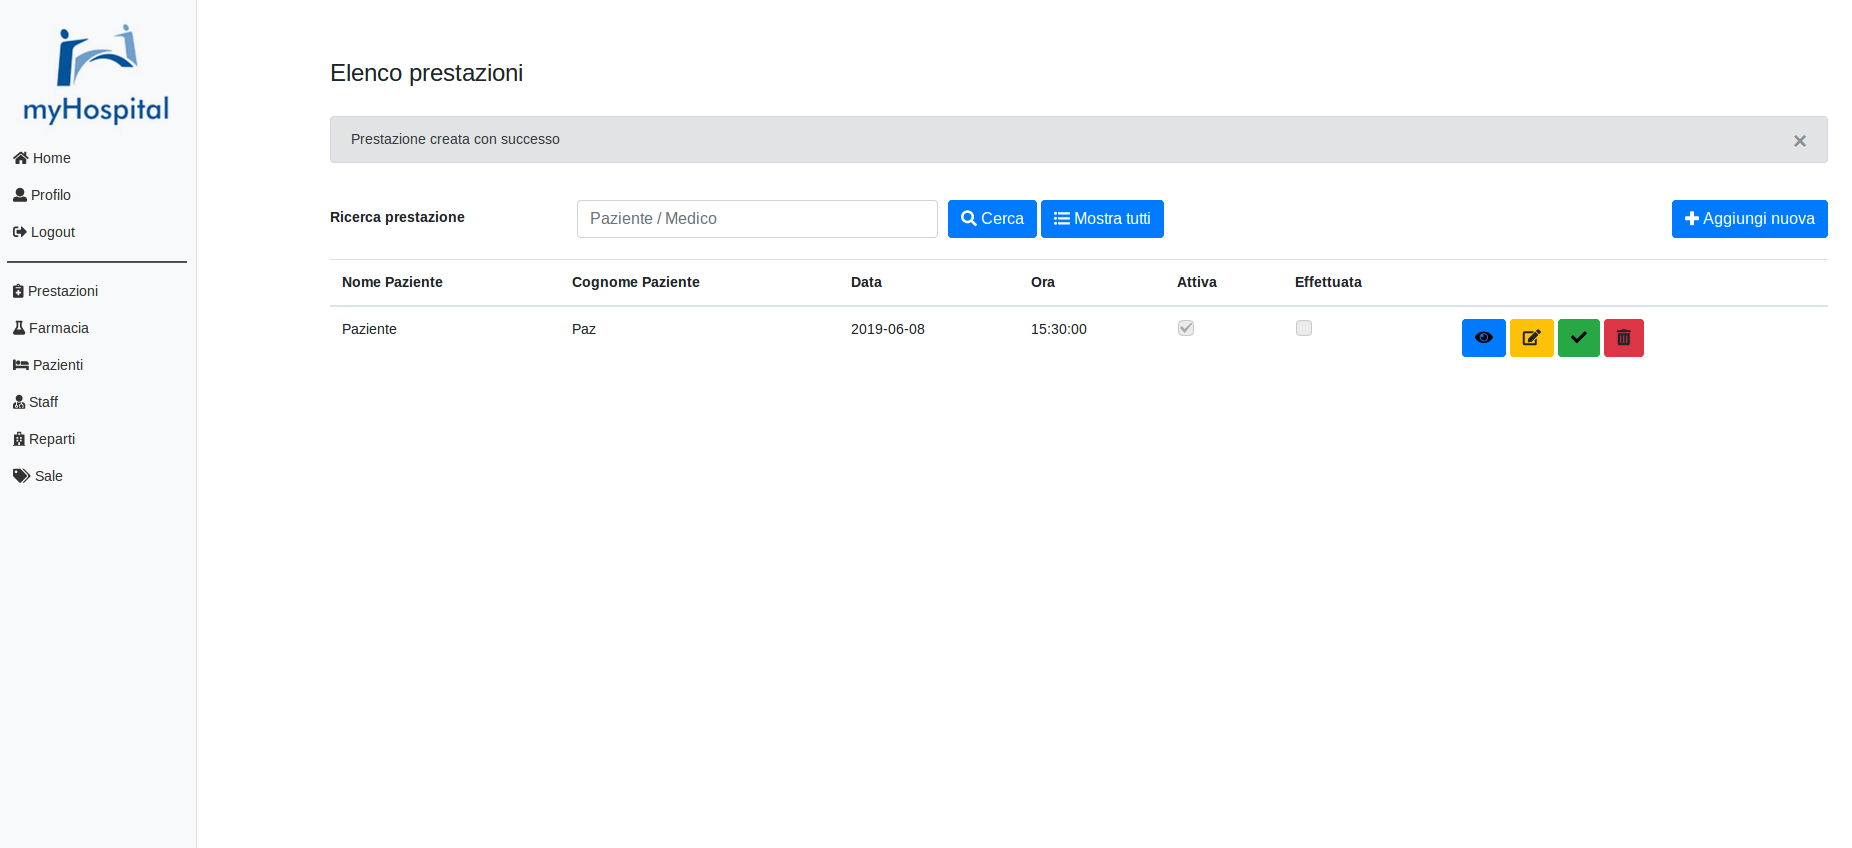
\includegraphics[scale=0.6]{grafica/ElencoPrestazioni}
\caption{Elenco delle prestazioni.}
\end{center}
\end{figure}
\end{landscape}

\begin{landscape}
\begin{figure}[H]
\begin{center}
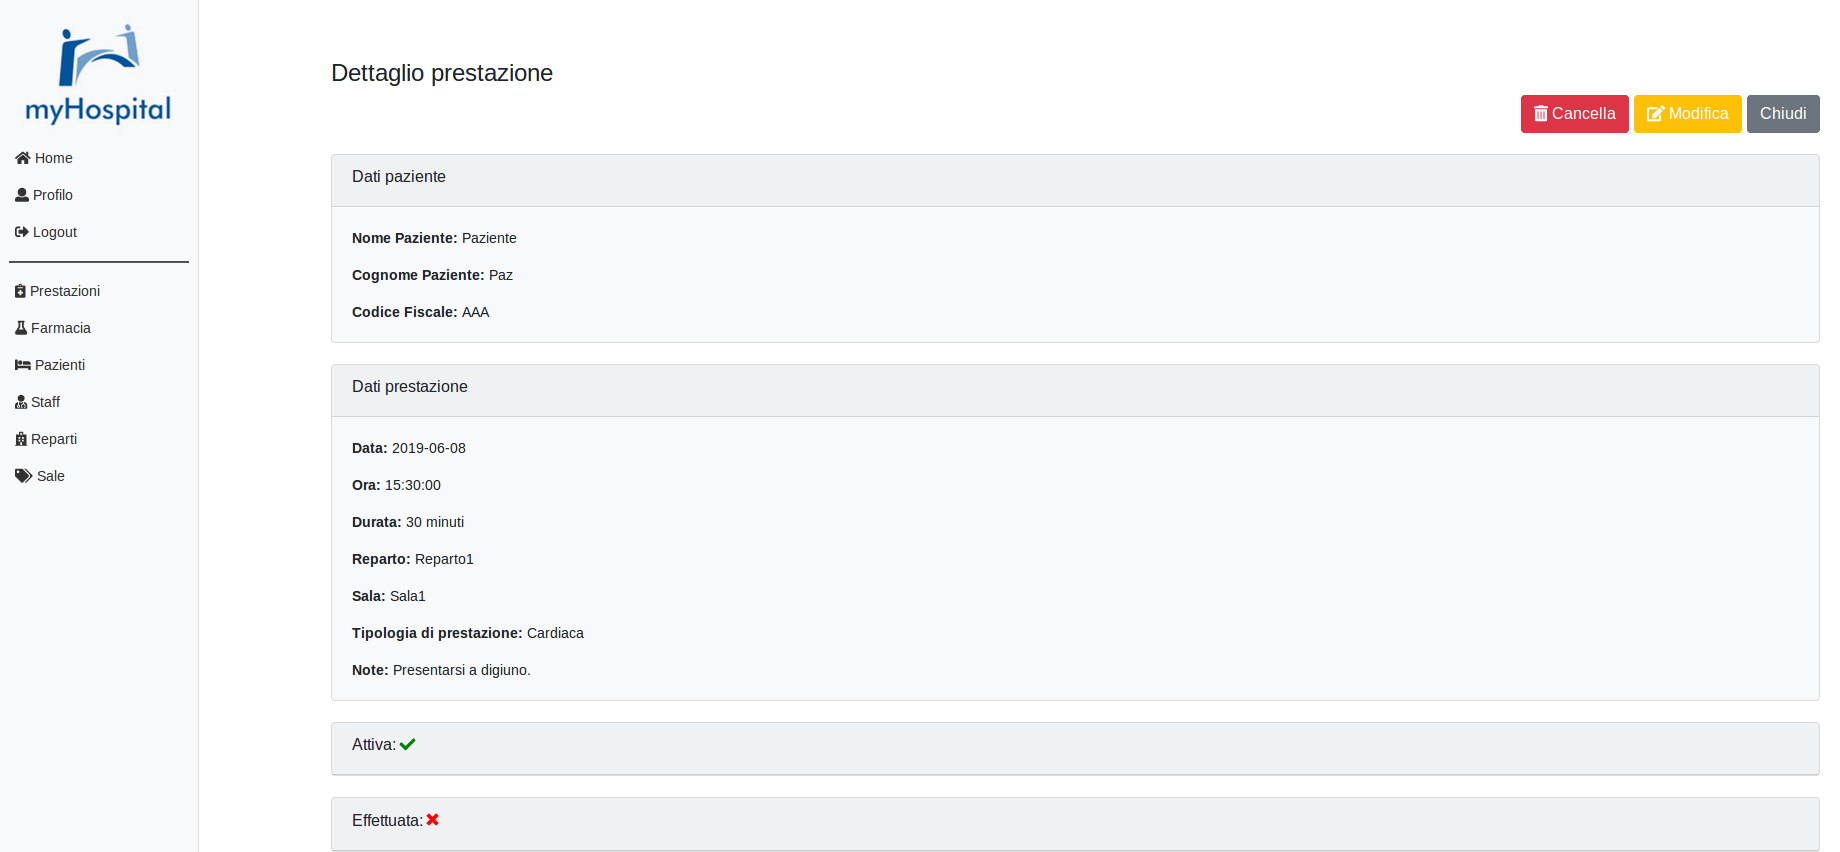
\includegraphics[scale=0.6]{grafica/DettaglioPrestazione}
\caption{Dettaglio della prestazione.}
\end{center}
\end{figure}
\end{landscape}

%%%%%%%%%%%%%%%%%%%%%%%%% BIBLIOGRAFIA


%%% End document
\end{document}